%%%%%%%%%%%%%%%%%%%%%%%%%%%%%%%%%%%%%%%%%
% The Legrand Orange Book
% LaTeX Template
% Version 1.4 (12/4/14)
%
% This template has been downloaded from:
% http://www.LaTeXTemplates.com
%
% Original author:
% Mathias Legrand (legrand.mathias@gmail.com)
%
% License:
% CC BY-NC-SA 3.0 (http://creativecommons.org/licenses/by-nc-sa/3.0/)
%
% Compiling this template:
% This template uses biber for its bibliography and makeindex for its index.
% When you first open the template, compile it from the command line with the 
% commands below to make sure your LaTeX distribution is configured correctly:
%
% 1) pdflatex main
% 2) makeindex main.idx -s StyleInd.ist
% 3) biber main
% 4) pdflatex main x 2
%
% After this, when you wish to update the bibliography/index use the appropriate
% command above and make sure to compile with pdflatex several times 
% afterwards to propagate your changes to the document.
%
% This template also uses a number of packages which may need to be
% updated to the newest versions for the template to compile. It is strongly
% recommended you update your LaTeX distribution if you have any
% compilation errors.
%
% Important note:
% Chapter heading images should have a 2:1 width:height ratio,
% e.g. 920px width and 460px height.
%
%%%%%%%%%%%%%%%%%%%%%%%%%%%%%%%%%%%%%%%%%

%----------------------------------------------------------------------------------------
%	PACKAGES AND OTHER DOCUMENT CONFIGURATIONS
%----------------------------------------------------------------------------------------

\documentclass[11pt,fleqn]{book} % Default font size and left-justified equations

\usepackage[top=3cm,bottom=3cm,left=3.2cm,right=3.2cm,headsep=10pt,a4paper]{geometry} % Page margins

\usepackage{xcolor} % Required for specifying colors by name
\definecolor{ocre}{RGB}{243,102,25} % Define the orange color used for highlighting throughout the book

% Font Settings
\usepackage{avant} % Use the Avantgarde font for headings
%\usepackage{times} % Use the Times font for headings
\usepackage{mathptmx} % Use the Adobe Times Roman as the default text font together with math symbols from the Sym­bol, Chancery and Com­puter Modern fonts

%\usepackage{microtype} % Slightly tweak font spacing for aesthetics
\usepackage[utf8]{inputenc} % Required for including letters with accents
%\usepackage[T1]{fontenc} % Use 8-bit encoding that has 256 glyphs
\usepackage[UTF8,fontset=mac]{ctex}
%\ctexset{today=small}
\usepackage{fontawesome}
%\usepackage[colorlinks,linkcolor=red]{hyperref}
\usepackage[skip=5pt]{caption}
\usepackage{subcaption}

% Bibliography
\usepackage[style=alphabetic,sorting=nyt,sortcites=true,autopunct=true,babel=hyphen,hyperref=true,abbreviate=false,backref=true,backend=biber]{biblatex}
\addbibresource{bibliography.bib} % BibTeX bibliography file
\defbibheading{bibempty}{}

% Index
\usepackage{calc} % For simpler calculation - used for spacing the index letter headings correctly
\usepackage{makeidx} % Required to make an index
\makeindex % Tells LaTeX to create the files required for indexing

%----------------------------------------------------------------------------------------

%----------------------------------------------------------------------------------------
%	VARIOUS REQUIRED PACKAGES
%----------------------------------------------------------------------------------------
\usepackage{titlesec} % Allows customization of titles

\usepackage{graphicx} % Required for including pictures
\graphicspath{{Pictures/}} % Specifies the directory where pictures are stored

\usepackage{lipsum} % Inserts dummy text

\usepackage{tikz} % Required for drawing custom shapes

\usepackage[english]{babel} % English language/hyphenation

\usepackage{enumitem} % Customize lists
\setlist{nolistsep} % Reduce spacing between bullet points and numbered lists

\usepackage{booktabs} % Required for nicer horizontal rules in tables

\usepackage{eso-pic} % Required for specifying an image background in the title page

%----------------------------------------------------------------------------------------
%	MAIN TABLE OF CONTENTS
%----------------------------------------------------------------------------------------

\usepackage{titletoc} % Required for manipulating the table of contents

\contentsmargin{0cm} % Removes the default margin
% Chapter text styling
\titlecontents{chapter}[1.25cm] % Indentation
{\addvspace{15pt}\large\sffamily\bfseries} % Spacing and font options for chapters
{\color{ocre!60}\contentslabel[\Large\thecontentslabel]{1.25cm}\color{ocre}} % Chapter number
{}  
{\color{ocre!60}\normalsize\sffamily\bfseries\;\titlerule*[.5pc]{.}\;\thecontentspage} % Page number
% Section text styling
\titlecontents{section}[1.25cm] % Indentation
{\addvspace{5pt}\sffamily\bfseries} % Spacing and font options for sections
{\contentslabel[\thecontentslabel]{1.25cm}} % Section number
{}
{\sffamily\hfill\color{black}\thecontentspage} % Page number
[]
% Subsection text styling
\titlecontents{subsection}[1.25cm] % Indentation
{\addvspace{1pt}\sffamily\small} % Spacing and font options for subsections
{\contentslabel[\thecontentslabel]{1.25cm}} % Subsection number
{}
{\sffamily\;\titlerule*[.5pc]{.}\;\thecontentspage} % Page number
[] 

%----------------------------------------------------------------------------------------
%	MINI TABLE OF CONTENTS IN CHAPTER HEADS
%----------------------------------------------------------------------------------------

% Section text styling
\titlecontents{lsection}[0em] % Indendating
{\footnotesize\sffamily} % Font settings
{}
{}
{}

% Subsection text styling
\titlecontents{lsubsection}[.5em] % Indentation
{\normalfont\footnotesize\sffamily} % Font settings
{}
{}
{}
 
%----------------------------------------------------------------------------------------
%	PAGE HEADERS
%----------------------------------------------------------------------------------------

\usepackage{fancyhdr} % Required for header and footer configuration

\pagestyle{fancy}
\renewcommand{\chaptermark}[1]{\markboth{\sffamily\normalsize\bfseries\chaptername\ \thechapter.\ #1}{}} % Chapter text font settings
\renewcommand{\sectionmark}[1]{\markright{\sffamily\normalsize\thesection\hspace{5pt}#1}{}} % Section text font settings
\fancyhf{} \fancyhead[LE,RO]{\sffamily\normalsize\thepage} % Font setting for the page number in the header
\fancyhead[LO]{\rightmark} % Print the nearest section name on the left side of odd pages
\fancyhead[RE]{\leftmark} % Print the current chapter name on the right side of even pages
\renewcommand{\headrulewidth}{0.5pt} % Width of the rule under the header
\addtolength{\headheight}{2.5pt} % Increase the spacing around the header slightly
\renewcommand{\footrulewidth}{0pt} % Removes the rule in the footer
\fancypagestyle{plain}{\fancyhead{}\renewcommand{\headrulewidth}{0pt}} % Style for when a plain pagestyle is specified

% Removes the header from odd empty pages at the end of chapters
\makeatletter
\renewcommand{\cleardoublepage}{
\clearpage\ifodd\c@page\else
\hbox{}
\vspace*{\fill}
\thispagestyle{empty}
\newpage
\fi}

%----------------------------------------------------------------------------------------
%	THEOREM STYLES
%----------------------------------------------------------------------------------------

\usepackage{amsmath,amsfonts,amssymb,amsthm} % For math equations, theorems, symbols, etc

\newcommand{\intoo}[2]{\mathopen{]}#1\,;#2\mathclose{[}}
\newcommand{\ud}{\mathop{\mathrm{{}d}}\mathopen{}}
\newcommand{\intff}[2]{\mathopen{[}#1\,;#2\mathclose{]}}
\newtheorem{notation}{Notation}[chapter]

%%%%%%%%%%%%%%%%%%%%%%%%%%%%%%%%%%%%%%%%%%%%%%%%%%%%%%%%%%%%%%%%%%%%%%%%%%%
%%%%%%%%%%%%%%%%%%%% dedicated to boxed/framed environements %%%%%%%%%%%%%%
%%%%%%%%%%%%%%%%%%%%%%%%%%%%%%%%%%%%%%%%%%%%%%%%%%%%%%%%%%%%%%%%%%%%%%%%%%%
\newtheoremstyle{ocrenumbox}% % Theorem style name
{0pt}% Space above
{0pt}% Space below
{\normalfont}% % Body font
{}% Indent amount
{\small\bf\sffamily\color{ocre}}% % Theorem head font
{\;}% Punctuation after theorem head
{0.25em}% Space after theorem head
{\small\sffamily\color{ocre}\thmname{#1}\nobreakspace\thmnumber{\@ifnotempty{#1}{}\@upn{#2}}% Theorem text (e.g. Theorem 2.1)
\thmnote{\nobreakspace\the\thm@notefont\sffamily\bfseries\color{black}---\nobreakspace#3.}} % Optional theorem note
\renewcommand{\qedsymbol}{$\blacksquare$}% Optional qed square

\newtheoremstyle{blacknumex}% Theorem style name
{5pt}% Space above
{5pt}% Space below
{\normalfont}% Body font
{} % Indent amount
{\small\bf\sffamily}% Theorem head font
{\;}% Punctuation after theorem head
{0.25em}% Space after theorem head
{\small\sffamily{\tiny\ensuremath{\blacksquare}}\nobreakspace\thmname{#1}\nobreakspace\thmnumber{\@ifnotempty{#1}{}\@upn{#2}}% Theorem text (e.g. Theorem 2.1)
\thmnote{\nobreakspace\the\thm@notefont\sffamily\bfseries---\nobreakspace#3.}}% Optional theorem note

\newtheoremstyle{blacknumbox} % Theorem style name
{0pt}% Space above
{0pt}% Space below
{\normalfont}% Body font
{}% Indent amount
{\small\bf\sffamily}% Theorem head font
{\;}% Punctuation after theorem head
{0.25em}% Space after theorem head
{\small\sffamily\thmname{#1}\nobreakspace\thmnumber{\@ifnotempty{#1}{}\@upn{#2}}% Theorem text (e.g. Theorem 2.1)
\thmnote{\nobreakspace\the\thm@notefont\sffamily\bfseries---\nobreakspace#3.}}% Optional theorem note

%%%%%%%%%%%%%%%%%%%%%%%%%%%%%%%%%%%%%%%%%%%%%%%%%%%%%%%%%%%%%%%%%%%%%%%%%%%
%%%%%%%%%%%%% dedicated to non-boxed/non-framed environements %%%%%%%%%%%%%
%%%%%%%%%%%%%%%%%%%%%%%%%%%%%%%%%%%%%%%%%%%%%%%%%%%%%%%%%%%%%%%%%%%%%%%%%%%
\newtheoremstyle{ocrenum}% % Theorem style name
{5pt}% Space above
{5pt}% Space below
{\normalfont}% % Body font
{}% Indent amount
{\small\bf\sffamily\color{ocre}}% % Theorem head font
{\;}% Punctuation after theorem head
{0.25em}% Space after theorem head
{\small\sffamily\color{ocre}\thmname{#1}\nobreakspace\thmnumber{\@ifnotempty{#1}{}\@upn{#2}}% Theorem text (e.g. Theorem 2.1)
\thmnote{\nobreakspace\the\thm@notefont\sffamily\bfseries\color{black}---\nobreakspace#3.}} % Optional theorem note
\renewcommand{\qedsymbol}{$\blacksquare$}% Optional qed square
\makeatother

% Defines the theorem text style for each type of theorem to one of the three styles above
\newcounter{dummy} 
\numberwithin{dummy}{section}
\theoremstyle{ocrenumbox}
\newtheorem{theoremeT}[dummy]{Theorem}
\newtheorem{problem}{Problem}[chapter]
%\newtheorem{exerciseT}{Exercise}[chapter]
\newtheorem{tipT}{Tip}[chapter]
\theoremstyle{blacknumex}
\newtheorem{exampleT}{Example}[chapter]
\theoremstyle{blacknumbox}
\newtheorem{vocabulary}{Vocabulary}[chapter]
%\newtheorem{definitionT}{Definition}[section]
\newtheorem{recommendationT}{Recommendation}[section]
\newtheorem{corollaryT}[dummy]{Corollary}
\theoremstyle{ocrenum}
\newtheorem{proposition}[dummy]{Proposition}

%----------------------------------------------------------------------------------------
%	DEFINITION OF COLORED BOXES
%----------------------------------------------------------------------------------------

\RequirePackage[framemethod=default]{mdframed} % Required for creating the theorem, definition, exercise and corollary boxes

% Theorem box
\newmdenv[skipabove=7pt,
skipbelow=7pt,
backgroundcolor=black!5,
linecolor=ocre,
innerleftmargin=5pt,
innerrightmargin=5pt,
innertopmargin=5pt,
leftmargin=0cm,
rightmargin=0cm,
innerbottommargin=5pt]{tBox}

% Exercise box	  
\newmdenv[skipabove=7pt,
skipbelow=7pt,
rightline=false,
leftline=true,
topline=false,
bottomline=false,
backgroundcolor=ocre!10,
linecolor=ocre,
innerleftmargin=5pt,
innerrightmargin=5pt,
innertopmargin=5pt,
innerbottommargin=5pt,
leftmargin=0cm,
rightmargin=0cm,
linewidth=4pt]{eBox}	

% Definition box
\newmdenv[skipabove=7pt,
skipbelow=7pt,
rightline=false,
leftline=true,
topline=false,
bottomline=false,
linecolor=ocre,
innerleftmargin=5pt,
innerrightmargin=5pt,
innertopmargin=0pt,
leftmargin=0cm,
rightmargin=0cm,
linewidth=4pt,
innerbottommargin=0pt]{dBox}	

% Corollary box
\newmdenv[skipabove=7pt,
skipbelow=7pt,
rightline=false,
leftline=true,
topline=false,
bottomline=false,
linecolor=gray,
backgroundcolor=black!5,
innerleftmargin=5pt,
innerrightmargin=5pt,
innertopmargin=5pt,
leftmargin=0cm,
rightmargin=0cm,
linewidth=4pt,
innerbottommargin=5pt]{cBox}

% Creates an environment for each type of theorem and assigns it a theorem text style from the "Theorem Styles" section above and a colored box from above
\newenvironment{theorem}{\begin{tBox}\begin{theoremeT}}{\end{theoremeT}\end{tBox}}
%\newenvironment{exercise}{\begin{eBox}\begin{exerciseT}}{\hfill{\color{ocre}\tiny\ensuremath{\blacksquare}}\end{exerciseT}\end{eBox}}				  
\newenvironment{tips}{\begin{eBox}\begin{tipT}}{\hfill{\color{ocre}\tiny\ensuremath{\blacksquare}}\end{tipT}\end{eBox}}				  
%\newenvironment{definition}{\begin{dBox}\begin{definitionT}}{\end{definitionT}\end{dBox}}	
\newenvironment{recommendation}{\begin{dBox}\begin{recommendationT}}{\end{recommendationT}\end{dBox}}	
\newenvironment{example}{\begin{exampleT}}{\hfill{\tiny\ensuremath{\blacksquare}}\end{exampleT}}		
\newenvironment{corollary}{\begin{cBox}\begin{corollaryT}}{\end{corollaryT}\end{cBox}}	

%----------------------------------------------------------------------------------------
%	REMARK ENVIRONMENT
%----------------------------------------------------------------------------------------

\newenvironment{remark}{\par\vspace{10pt}\small % Vertical white space above the remark and smaller font size
\begin{list}{}{
\leftmargin=35pt % Indentation on the left
\rightmargin=25pt}\item\ignorespaces % Indentation on the right
\makebox[-2.5pt]{\begin{tikzpicture}[overlay]
\node[draw=ocre!60,line width=1pt,circle,fill=ocre!25,font=\sffamily\bfseries,inner sep=2pt,outer sep=0pt] at (-15pt,0pt){\textcolor{ocre}{R}};\end{tikzpicture}} % Orange R in a circle
\advance\baselineskip -1pt}{\end{list}\vskip5pt} % Tighter line spacing and white space after remark

%----------------------------------------------------------------------------------------
%	SECTION NUMBERING IN THE MARGIN
%----------------------------------------------------------------------------------------

\makeatletter
\renewcommand{\@seccntformat}[1]{\llap{\textcolor{ocre}{\csname the#1\endcsname}\hspace{1em}}}                    
\renewcommand{\section}{\@startsection{section}{1}{\z@}
{-4ex \@plus -1ex \@minus -.4ex}
{1ex \@plus.2ex }
{\normalfont\large\sffamily\bfseries}}
\renewcommand{\subsection}{\@startsection {subsection}{2}{\z@}
{-3ex \@plus -0.1ex \@minus -.4ex}
{0.5ex \@plus.2ex }
{\normalfont\sffamily\bfseries}}
\renewcommand{\subsubsection}{\@startsection {subsubsection}{3}{\z@}
{-2ex \@plus -0.1ex \@minus -.2ex}
{.2ex \@plus.2ex }
{\normalfont\small\sffamily\bfseries}}                        
\renewcommand\paragraph{\@startsection{paragraph}{4}{\z@}
{-2ex \@plus-.2ex \@minus .2ex}
{.1ex}
{\normalfont\small\sffamily\bfseries}}

%----------------------------------------------------------------------------------------
%	HYPERLINKS IN THE DOCUMENTS
%----------------------------------------------------------------------------------------

% For an unclear reason, the package should be loaded now and not later
\usepackage{hyperref}
\hypersetup{hidelinks,backref=true,pagebackref=true,hyperindex=true,colorlinks=false,breaklinks=true,urlcolor= ocre,bookmarks=true,bookmarksopen=false,pdftitle={Title},pdfauthor={Author}}

%----------------------------------------------------------------------------------------
%	CHAPTER HEADINGS
%----------------------------------------------------------------------------------------

% The set-up below should be (sadly) manually adapted to the overall margin page septup controlled by the geometry package loaded in the main.tex document. It is possible to implement below the dimensions used in the goemetry package (top,bottom,left,right)... TO BE DONE

\newcommand{\thechapterimage}{}
\newcommand{\chapterimage}[1]{\renewcommand{\thechapterimage}{#1}}

% Numbered chapters with mini tableofcontents
\def\thechapter{\arabic{chapter}}
\def\@makechapterhead#1{
\thispagestyle{empty}
{\centering \normalfont\sffamily
\ifnum \c@secnumdepth >\m@ne
\if@mainmatter
\startcontents
\begin{tikzpicture}[remember picture,overlay]
\node at (current page.north west)
{\begin{tikzpicture}[remember picture,overlay]
\node[anchor=north west,inner sep=0pt] at (0,0) {\includegraphics[width=\paperwidth]{\thechapterimage}};
%%%%%%%%%%%%%%%%%%%%%%%%%%%%%%%%%%%%%%%%%%%%%%%%%%%%%%%%%%%%%%%%%%%%%%%%%%%%%%%%%%%%%
% Commenting the 3 lines below removes the small contents box in the chapter heading
\fill[color=ocre!10!white,opacity=.6] (1cm,0) rectangle (8cm,-7cm);
\node[anchor=north west] at (1.1cm,.35cm) {\parbox[t][8cm][t]{6.5cm}{\huge\bfseries\flushleft \printcontents{l}{1}{\setcounter{tocdepth}{2}}}};
\draw[anchor=west] (5cm,-9cm) node [rounded corners=20pt,fill=ocre!10!white,text opacity=1,draw=ocre,draw opacity=1,line width=1.5pt,fill opacity=.6,inner sep=12pt]{\huge\sffamily\bfseries\textcolor{black}{\thechapter. #1\strut\makebox[22cm]{}}};
%%%%%%%%%%%%%%%%%%%%%%%%%%%%%%%%%%%%%%%%%%%%%%%%%%%%%%%%%%%%%%%%%%%%%%%%%%%%%%%%%%%%%
\end{tikzpicture}};
\end{tikzpicture}}
\par\vspace*{230\p@}
\fi
\fi}

% Unnumbered chapters without mini tableofcontents (could be added though) 
\def\@makeschapterhead#1{
\thispagestyle{empty}
{\centering \normalfont\sffamily
\ifnum \c@secnumdepth >\m@ne
\if@mainmatter
\begin{tikzpicture}[remember picture,overlay]
\node at (current page.north west)
{\begin{tikzpicture}[remember picture,overlay]
\node[anchor=north west,inner sep=0pt] at (0,0) {\includegraphics[width=\paperwidth]{\thechapterimage}};
\draw[anchor=west] (5cm,-9cm) node [rounded corners=20pt,fill=ocre!10!white,fill opacity=.6,inner sep=12pt,text opacity=1,draw=ocre,draw opacity=1,line width=1.5pt]{\huge\sffamily\bfseries\textcolor{black}{#1\strut\makebox[22cm]{}}};
\end{tikzpicture}};
\end{tikzpicture}}
\par\vspace*{230\p@}
\fi
\fi
}
\makeatother
 % Insert the commands.tex file which contains the majority of the structure behind the template

\begin{document}

%----------------------------------------------------------------------------------------
%	TITLE PAGE
%----------------------------------------------------------------------------------------

\begingroup
\thispagestyle{empty}
\AddToShipoutPicture*{\put(6,5){
\includegraphics[scale=1]{background}}} % Image background
\centering
\vspace*{8cm}
\par\normalfont\fontsize{35}{35}\sffamily\selectfont
Linux \faLinux\ Mac \faApple\ Windows \faWindows 高效开源免费工具集\par % Book title
\vspace*{0.5cm}
{\huge \faWeibo 优天人 \\ 2016 年1 月}\par % Author name
\endgroup

%----------------------------------------------------------------------------------------
%	COPYRIGHT PAGE
%----------------------------------------------------------------------------------------

\newpage
~\vfill
\thispagestyle{empty}

\noindent Copyright \copyright\ 2016 优天人\\ % Copyright notice

\noindent \textsc{Published by 优天人}\\ % Publisher

\noindent \textsc{ask.fm/youtianren}\\ % URL

\noindent                                                                                        本文所有文字内容均归作者优天人所有,虽然不是真正有思想力度的东西,但是作者还是希望能帮到一些人,
所以在此特别声明:本册所载内容随便转发,无需打招呼,无需署名,并且感谢每一位传播者。乐于传播分享
是一种境界,作者还认为能帮助人就是一种能力,这种能力往往被绝大多人所忽略,希望每个人都能发掘出自
己的这种能力。 如有疑问请到这里 \href{weibo.com/u/2635198437}{\faWeibo 优天人} 发问,但是作者时间精力有限,不能保证及时回复。
\\
%\noindent Licensed under the Creative Commons Attribution-NonCommercial 3.0 Unported License (the ``License''). You may not use this file except in compliance with the License. You may obtain a copy of the License at \url{http://creativecommons.org/licenses/by-nc/3.0}. Unless required by applicable law or agreed to in writing, software distributed under the License is distributed on an \textsc{``as is'' basis, without warranties or conditions of any kind}, either express or implied. See the License for the specific language governing permissions and limitations under the License.\\ % License information

\noindent \textit{First draft, January 2016} % Printing/edition date

%----------------------------------------------------------------------------------------
%	TABLE OF CONTENTS
%----------------------------------------------------------------------------------------

\chapterimage{chapter_head_1.pdf} % Table of contents heading image

\pagestyle{empty} % No headers

\tableofcontents % Print the table of contents itself

\cleardoublepage % Forces the first chapter to start on an odd page so it's on the right

\pagestyle{fancy} % Print headers again

%----------------------------------------------------------------------------------------
%	CHAPTER 0
%----------------------------------------------------------------------------------------

\chapterimage{chapter_head_2.pdf} % Chapter heading image

\chapter{Preface}\index{Preface序言}

%-----------------------------------------------------------------------
\section{动机}\index{Motivation}\index{Preface动机}
本书成因在于作者喜欢折腾,作为一名理科学生,尤其喜欢折腾一些电脑之类的东西。
现在也记不清刚上大学那会儿是怎样接触到Linux的了,不过当时的兴趣盎然依然记忆犹新,
有时候装Linux系统折腾的一夜不睡觉,只为给Linux系统连上网。作为一个从农村里走出的孩子,
对电脑完全是小白一个,当时对新事物的好奇让我充满了战斗力,呆在宿舍里不吃饭却一直研究怎么在虚拟机
里装系统,怎么给黑莓刷机。一个学物理的宅男,平时没啥娱乐活动,所有时间都在折腾着电脑,
研究一些软件怎么用,研究Linux系统有多酷炫。时光荏苒,现在都读到博士了,不出国的话,应该博士毕业了,现在还在痴迷着技术,喜欢尝鲜各种科技电子产品。

回到正题,本文并非技术文档,只是根据作者的经历经验,记录的作者自己认为好用的工具,具体技术问题,
还需要各位读者去看官方文档或者论坛去找答案。所以本文的意义更多在于,当你需要完成某个任务不知道
该用什么工具时,当你想要找一个高效率的工具去完成工作时,或者只是出于兴趣想了解更多成为一个百科时
,你都可以来这儿看看,说不定就有意外的收获。

本文分为三个部分,Linux,Mac和Windows,实际上,很多开源工具都有三个系统的对应版本,虽然是同一
个软件,但是在不同都系统中用户体验或者说工作效率真的可能差别很大,一般来讲,开源工具是伴随Linux系统的,所以常常是在Linux系统下能给人以最好的体验和工作效率,这也是作者的主要工作环境,Mac作为Unix
系统,如果你能稍作努力也常常很高效,至于Windows系统我也很喜欢,只是更多用来娱乐而不是工作。
下面可以初探一下三个系统的外观,显然Linux简洁无比。

\begin{figure}[htpb]
  \centering
  \includegraphics[width=\textwidth]{mac}
  \caption{Mac OS X El Capitan}
  \label{fig:mac}
\end{figure}
\begin{figure}[htpb]
  \centering
  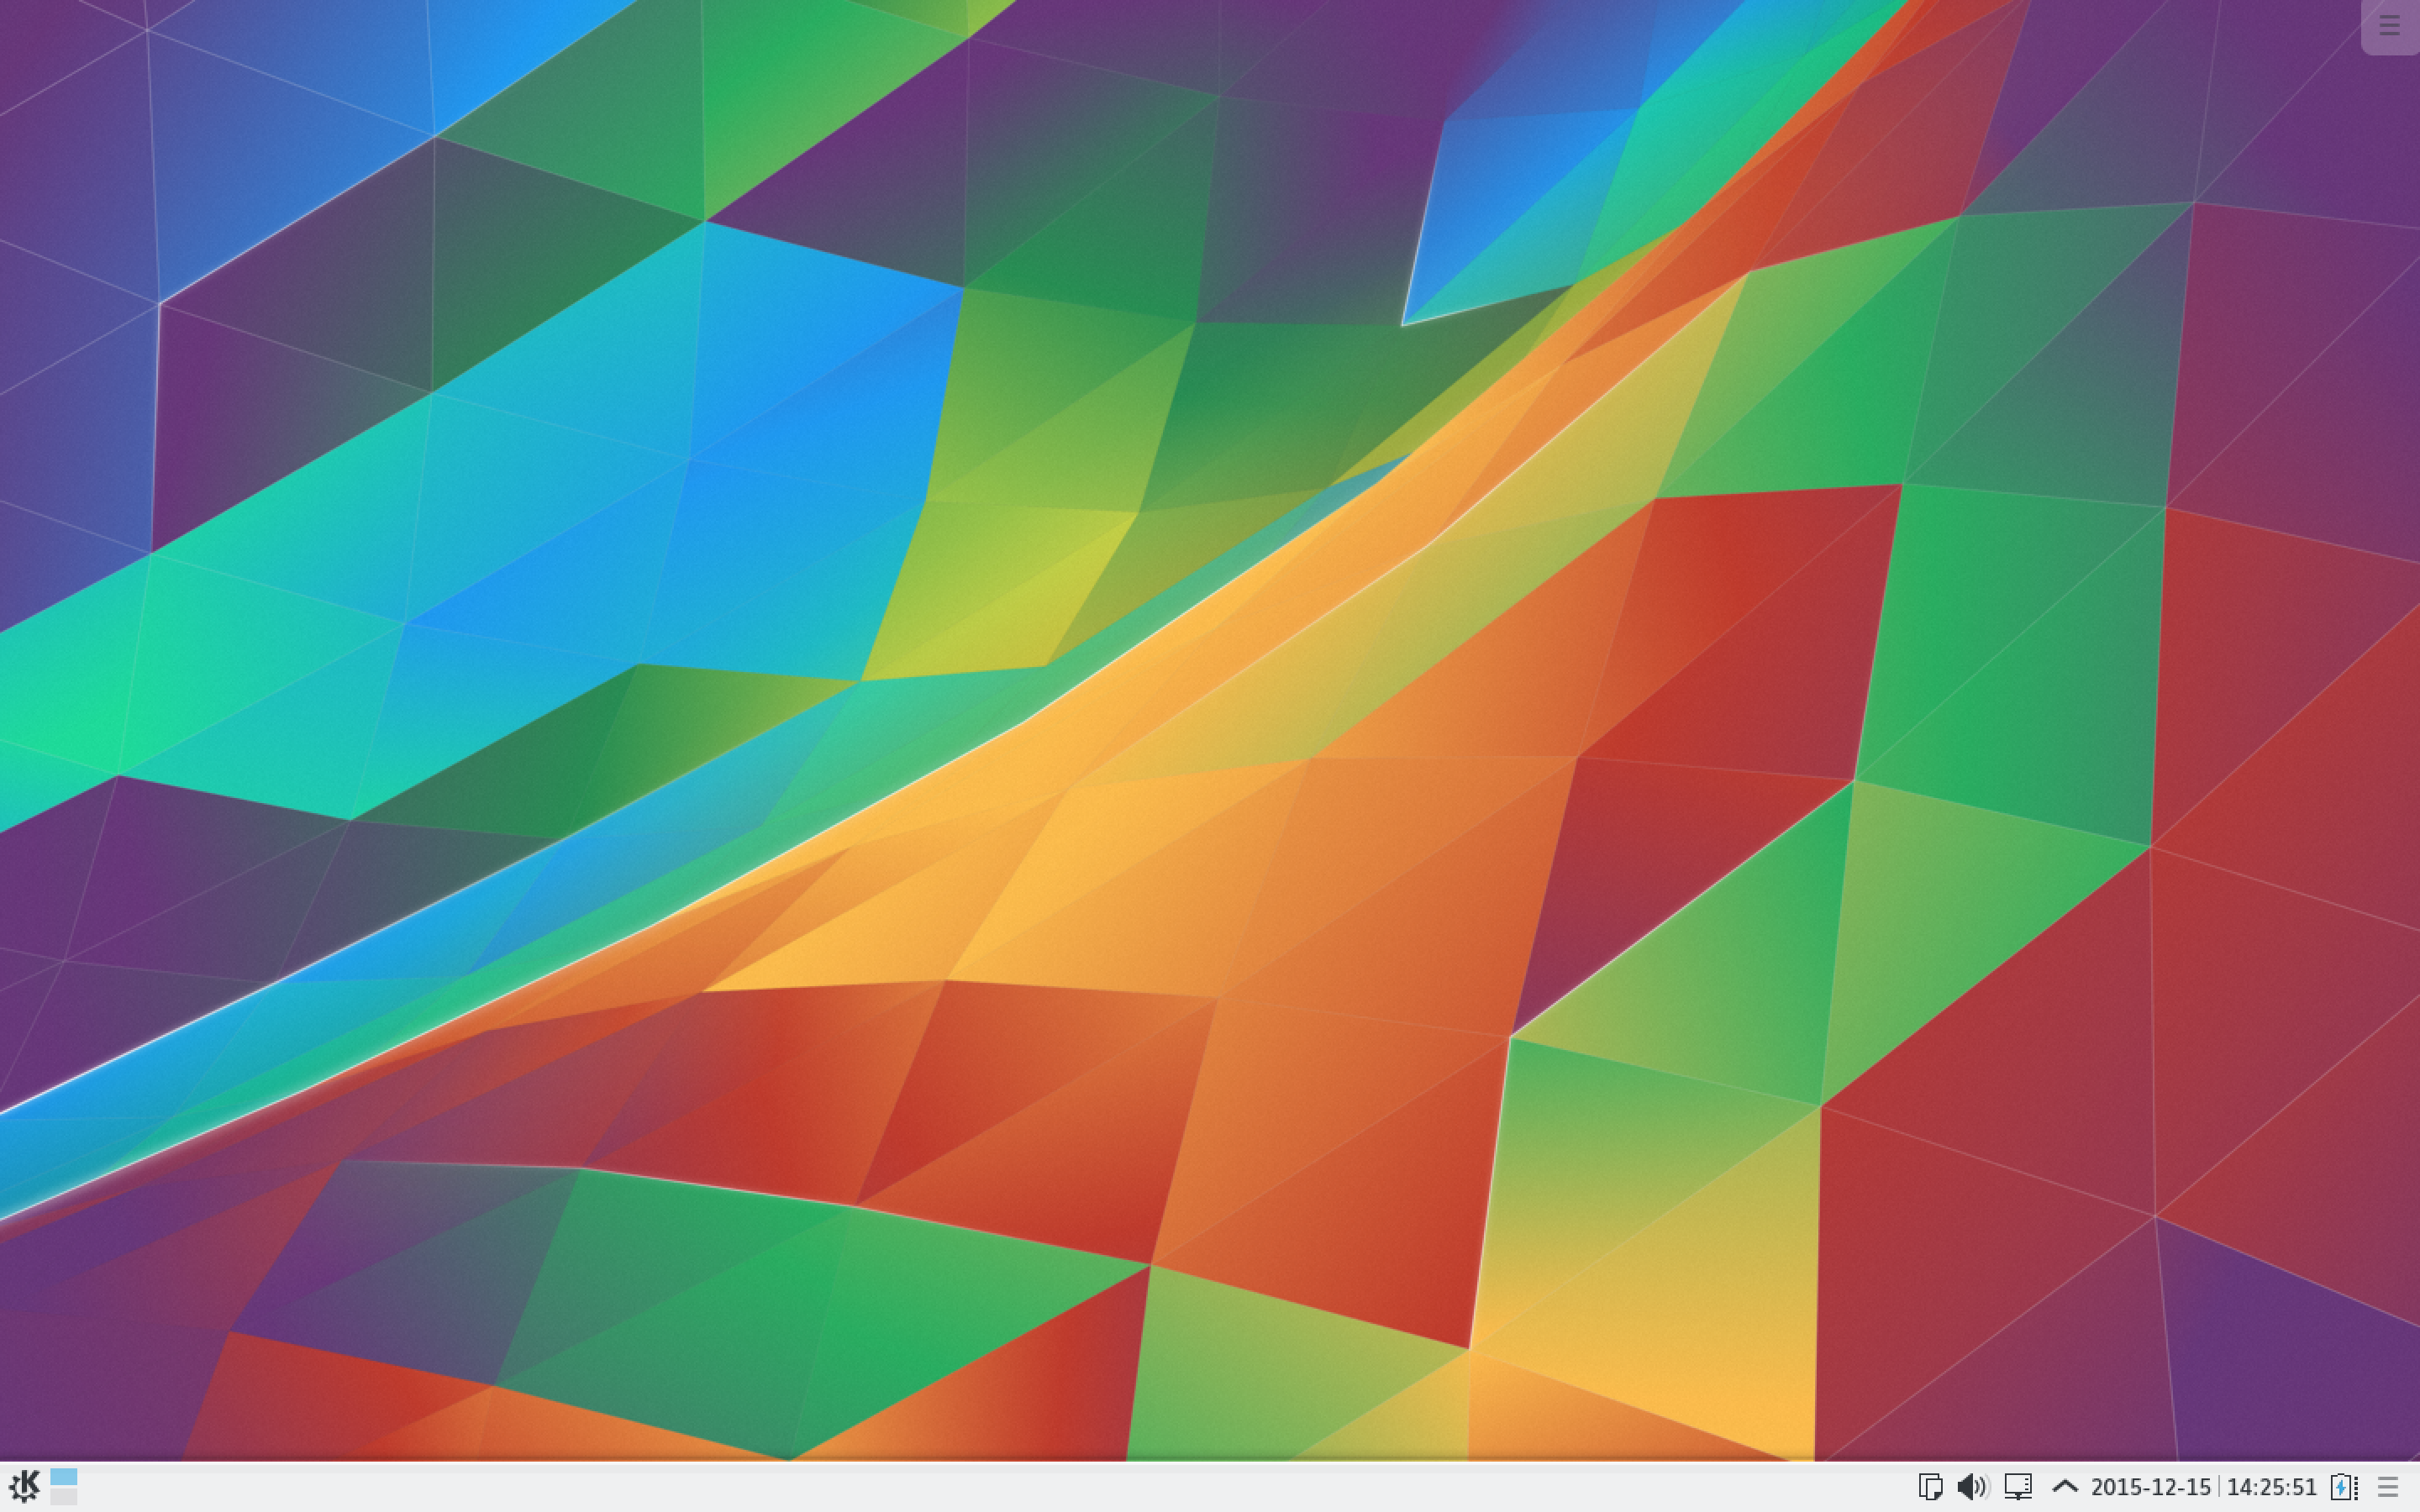
\includegraphics[width=\textwidth]{kde}
  \caption{Kubuntu 15.10 Wily werewolf}
  \label{fig:kde}
\end{figure}
\begin{figure}[htpb]
  \centering
  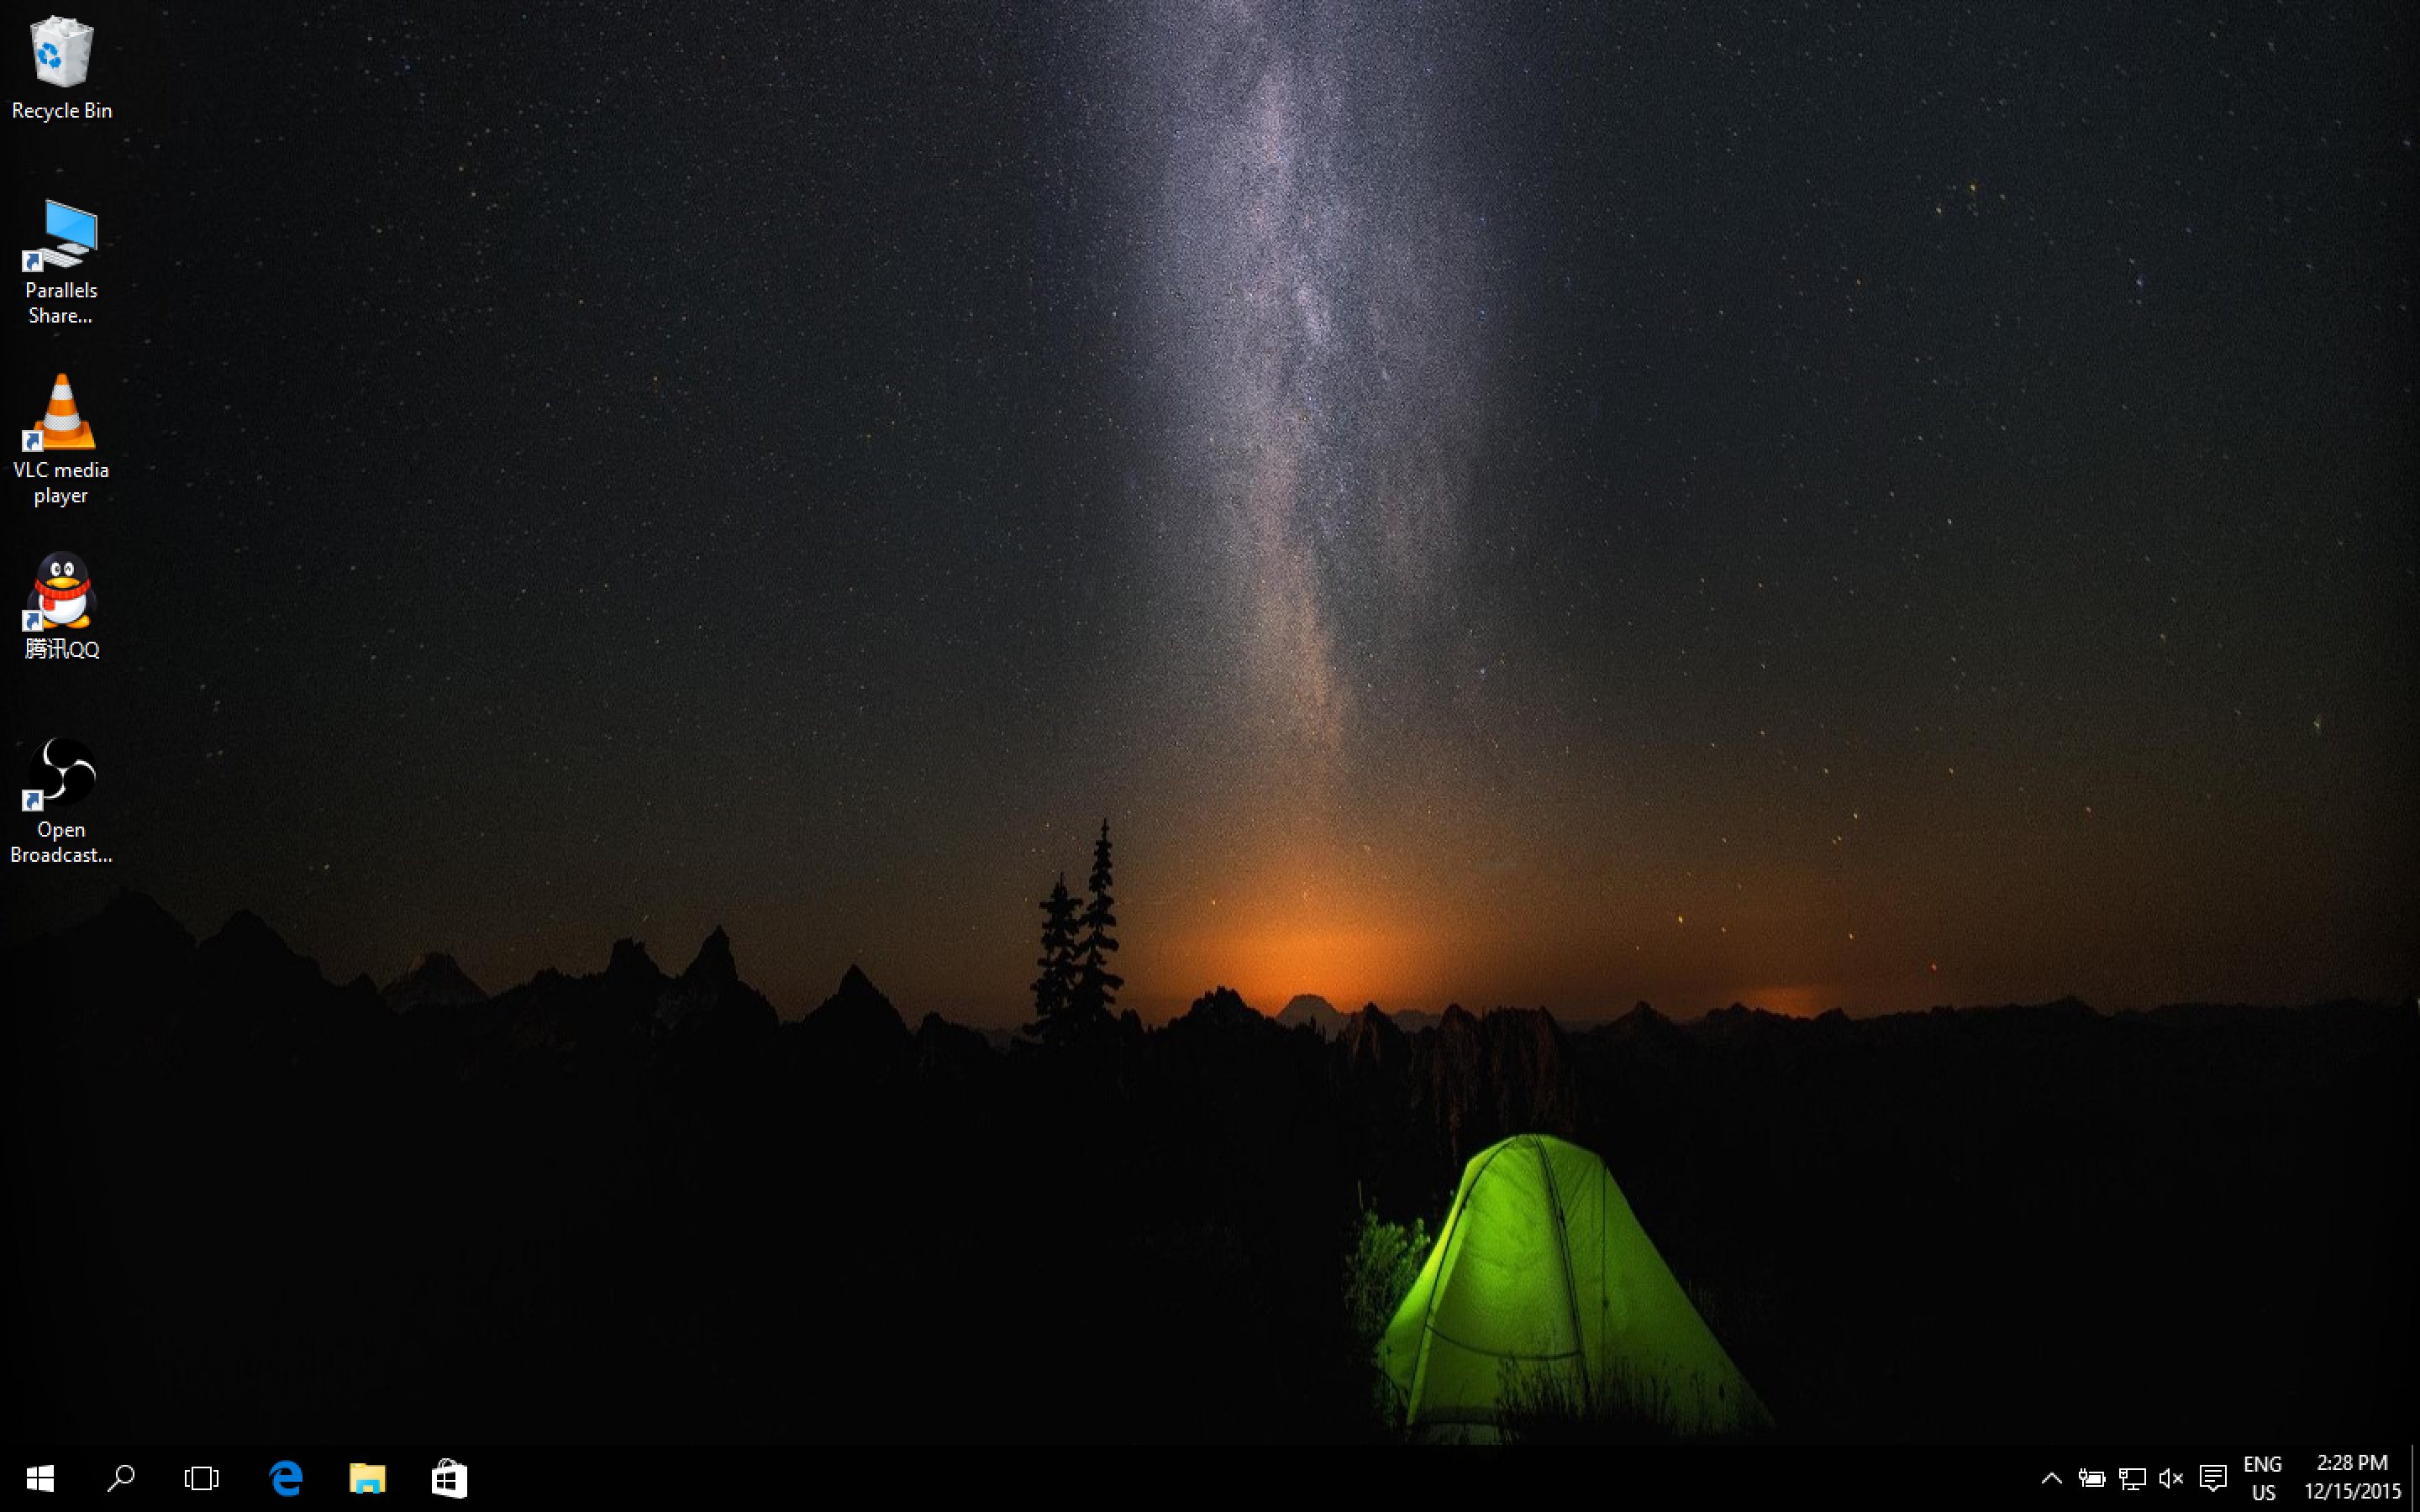
\includegraphics[width=\textwidth]{win10}
  \caption{Windows 10}
  \label{fig:win10}
\end{figure}

%-----------------------------------------------------------------------
\section{再一点说明}\index{Announcement}\index{Preface再一点说明}
由于本册主要目的在于介绍工具应用,因此关于系统方面并没有介绍,假设你已经熟悉了系统安装,当然这里
主要是指Linux系统的安装,不过现在系统安装相当简单,不像几年前安装时那么麻烦,特别是多系统安装,
常常遇到安装一个系统另一个系统启动时找不到了。我想能折腾系统的人一定具备一定的解决问题的能力,
善于运用搜索工具能帮助你节省大量时间。不要拘泥于百度和一些中文论坛,很多解决方案可以英文找到。
比如StackExchange \faStackExchange,stackoverflow \faStackOverflow,Google Group \faGroup
等论坛,如果不能用Google \faGoogle,可以试试Bing,Yahoo \faYahoo 等搜索。

本文按照常用系统分类了三个板块,显然这个循序是按照作者自己的喜好进行的,由于作者喜欢Linux作为工作
的首选系统,对它的喜爱程度到了无以复加的地步,这是由于Linux系统强大的生产力,十分灵活的定制性,
作者尤其钟情于它的大量快捷键定制,平日里作者从来不用鼠标,全键盘\faKeyboardO 操作的效率比用鼠标
\faMousePointer 点击大大提高。

实际上开源工具往往是跨平台的,很多都同时有三个系统的对应版本,也许使用逻辑稍有区别,但是功能上
往往差别不大,但是常常是Linux平台下效率高些。由于是按照系统分类的而不是按照工具类别分类的,所以
会有很多重合的工具介绍,也许下个版本会改用按照工具分类更合理些。

大体上,作者更偏爱openSUSE一些,虽然其他Linux版本如Ubuntu,Fedora,Linux Mint,Scientific Linux 
也用过,但是时间都不太长,而openSUSE却是更年累月的在使用,如果但就默认桌面的使用上来说,Fedora
感觉体验上是最快的,Ubuntu是支持最好资源最丰富的,openSUSE是最漂亮的, 是的,作者喜欢KDE桌面多一
些,所以最后看看作者工作的openSUSE桌面吧\faSmileO。

\begin{figure}[!ht]
  \centering
  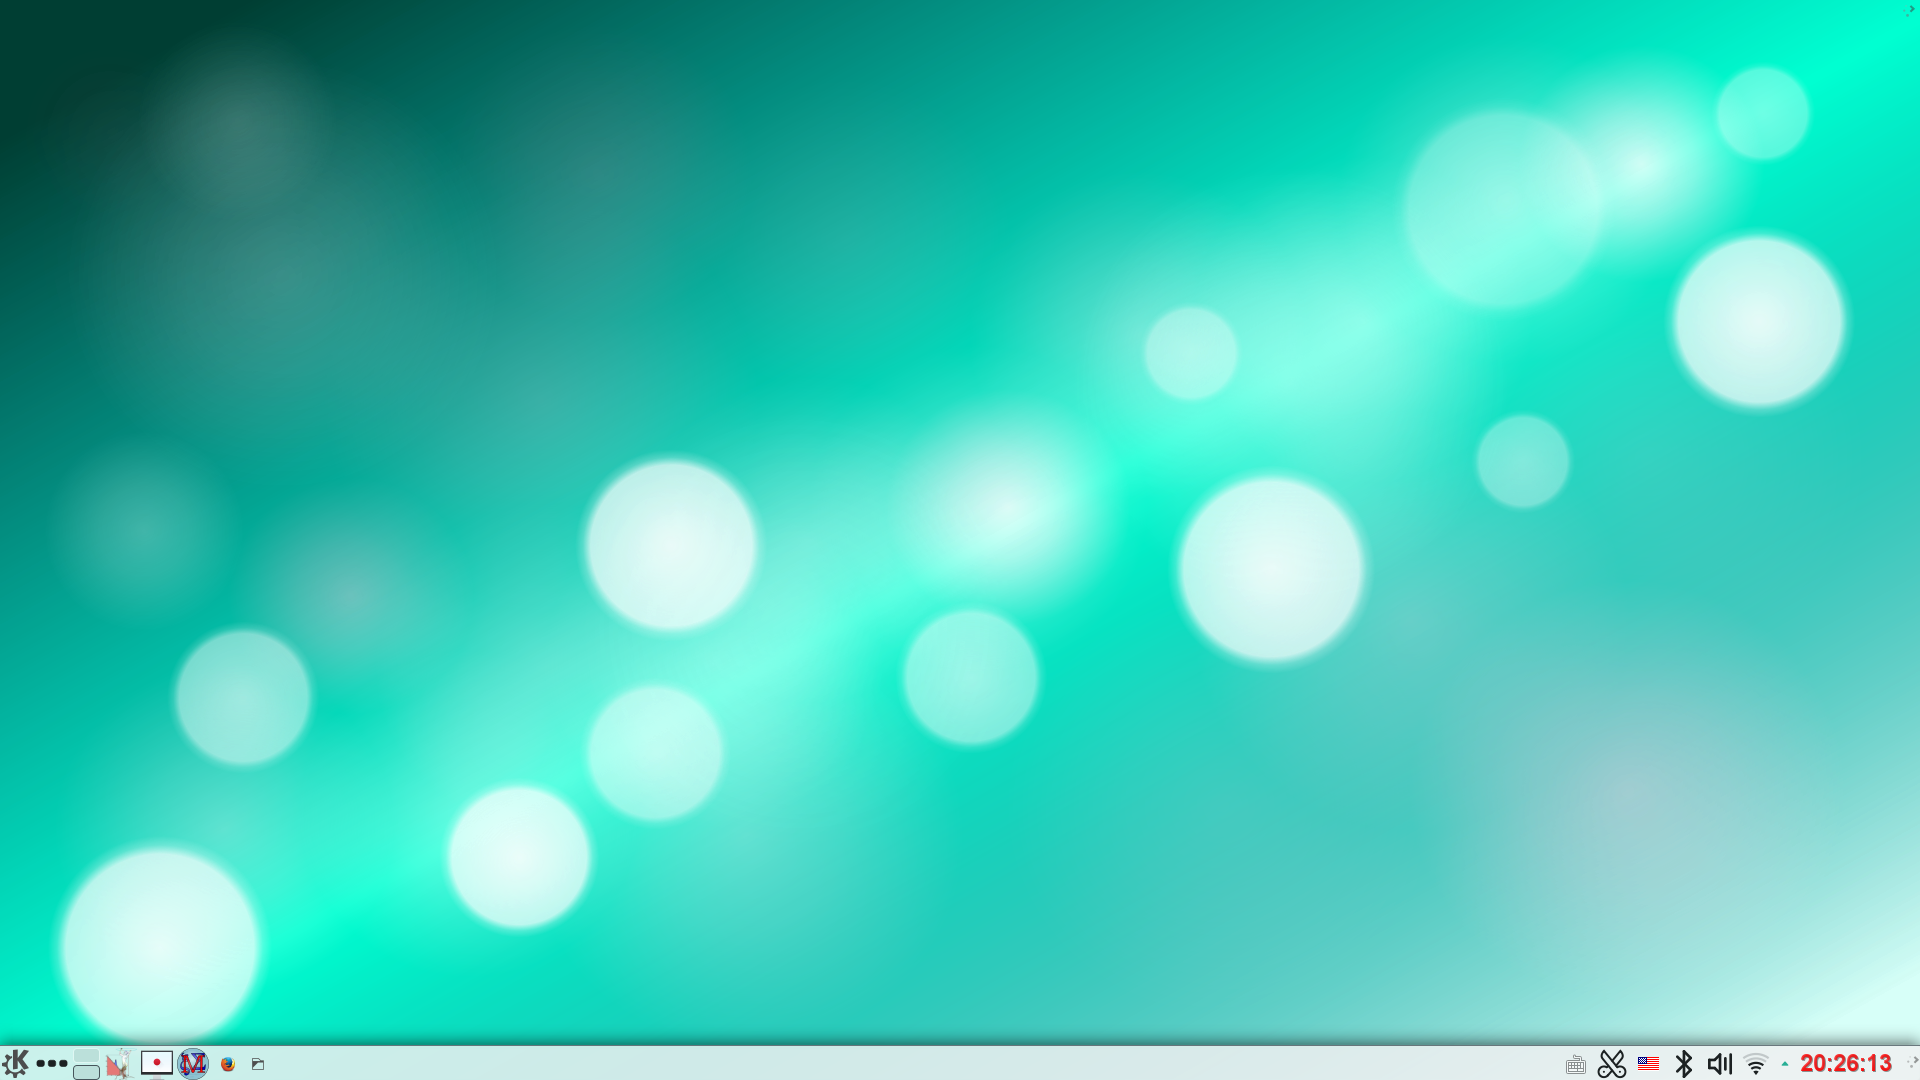
\includegraphics[width=\textwidth]{opensuse}
  \caption{openSUSE 13.2}
  \label{fig:opensuse1}
\end{figure}

\begin{figure}[!h]
  \centering
  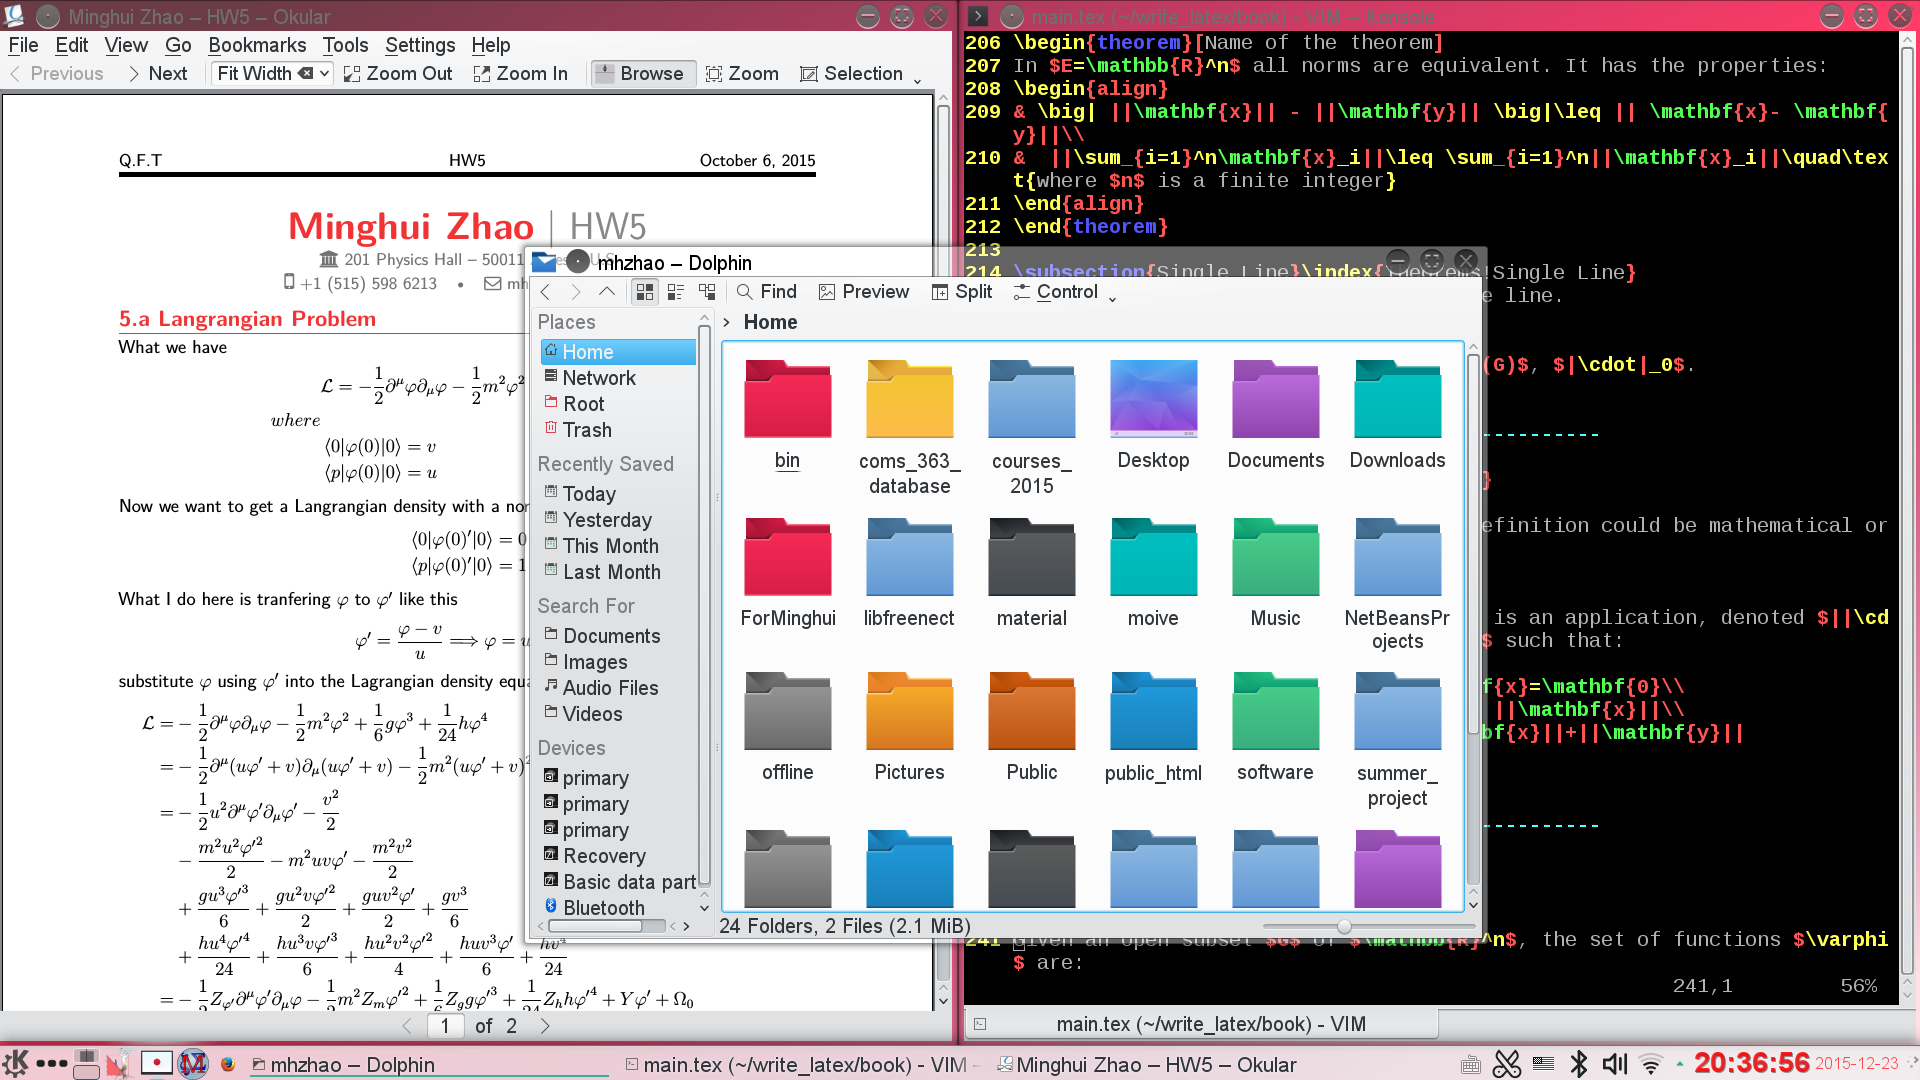
\includegraphics[width=\textwidth]{opensuse2}
  \caption{openSUSE 13.2}
  \label{fig:oepnsuse2}
\end{figure}

\begin{tips}
本册的写作是在作者的Winter Break期间,时间并不长,所以很多方面涉及不到,主要还是基于作者自己的
使用经验和常用软件,也为作者日后装新系统配置做个参考。这里还有很多没有日常软件没有涉及到,比如,
邮件收发,日常管理软件如note、reminder,联系人管理等,我一般使用KDE桌面自带的一套软件如Knotes,
Kmail, Kcontact等,感觉到非常好用,另外如虚拟机软件等开源的也就VirtualBox可选,所以都不再赘述了。
\end{tips}
%----------------------------------------------------------------------------------------
%	CHAPTER 1
%----------------------------------------------------------------------------------------

%\chapterimage{chapter_head_2.pdf} % Chapter heading image
\chapterimage{plasma} % Chapter heading image

\chapter{Linux \texorpdfstring{\faLinux}{world}}\index{Linux}

%-----------------------------------------------------------------------
\section{Linux版本选择}\index{Distributions of Linux}\index{Linux版本选择}

实际上Linux对于每一个人来说并不陌生,比如大家用的手机操作系统Android就是Linux众多分支中的一支,
由于Linux版本众多,对于刚入门的人选择哪个版本往往很困惑,除了软件包管理机制不同外,实际上它们用起
来并无实质上的区别,这里作者还是给出Top 10的选项,如果你还是难以抉择,那就听我的建议选择
Linux Mint或者openSUSE吧。


\includegraphics[width=0.3\textwidth]{Linux_Mint_logo}

\includegraphics[width=0.3\textwidth]{Ubuntu_logo}

\includegraphics[width=0.3\textwidth]{Mageia_logo}


\includegraphics[width=0.3\textwidth]{OpenSUSE_logo}
\hspace{1.2cm}

\includegraphics[width=0.5\textwidth]{Freebsd_logo}


\includegraphics[width=0.3\textwidth]{Fedora_logo}

\includegraphics[width=0.3\textwidth]{Arch_Linux_logo}

\includegraphics[width=0.3\textwidth]{Centos-logo}


\includegraphics[width=0.3\textwidth]{PCLinuxOS_logo}
\hspace{0.5cm}

\includegraphics[width=0.2\textwidth]{Debian-OpenLogo}
\hspace{0.5cm}
\includegraphics[width=0.3\textwidth]{Slackware_logo}

%-------------------------------------------------------
\subsection{Linux Mint}\index{Mint}\index{Linux Mint}
Linux Mint最初是由一位居于爱尔兰的法国IT专家Clement Lefebvre于2006年发起的基于Ubuntu的一个Linux
分支版本。尽管 Linux Mint是免费的,但是它的项目团队靠着捐赠、广告和专业支持服务获得收入。
它并没有固定的发行日期 ,不过一般它会在Ubuntu长期支持版本发布几周后发行新版本。
它有两个主要桌面环境,MATE和Cinnamon。

\noindent
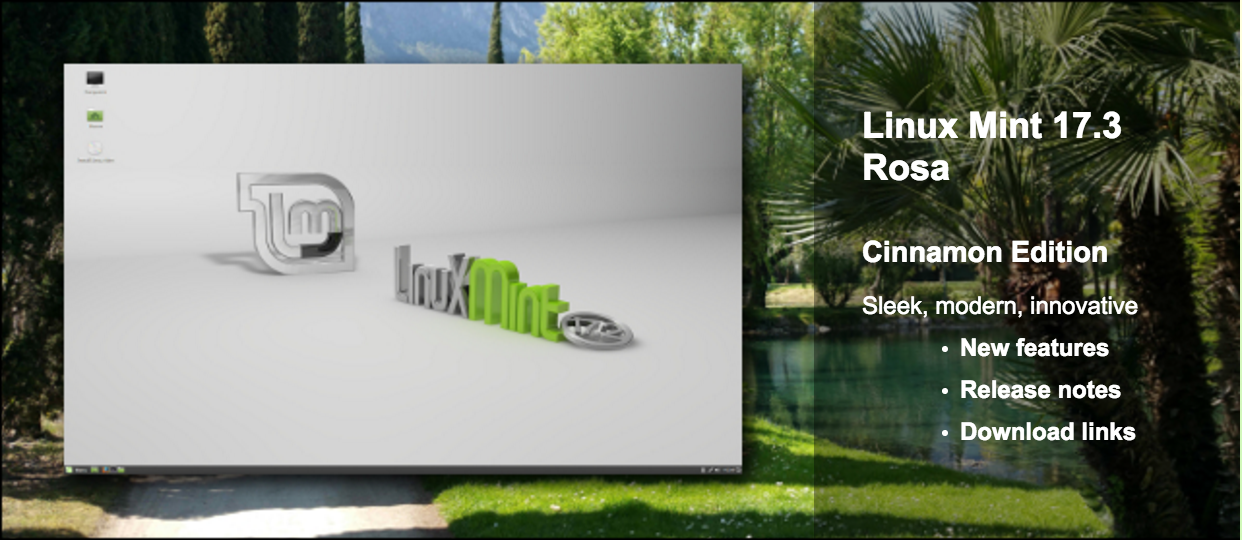
\includegraphics[width=0.5\textwidth]{Mint_cinnamon}
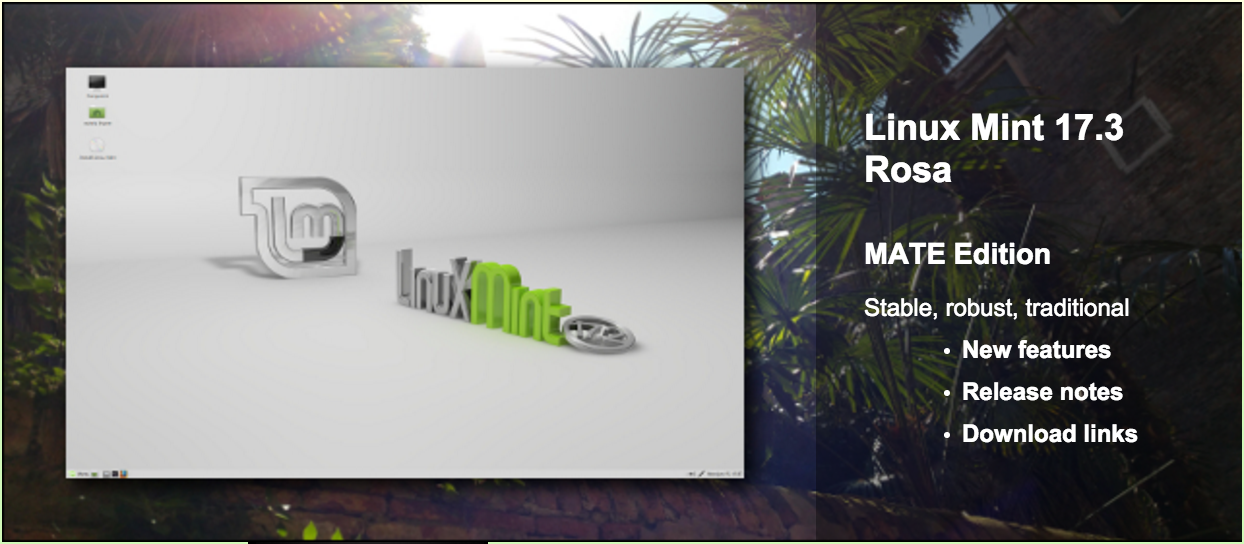
\includegraphics[width=0.5\textwidth]{Mint_mate}

\begin{itemize}
  \item \textbf{优点:}非常出色的原生支持工具,大量的用户友好优化,开放式接纳用户建议。
  \item \textbf{不足:}社区版本并不是总是采用最新的技术特性,也不发布安全建议。
  \item \textbf{软件包管理:}Advanced Package Tool (APT) 工具,采用DEB封装包(兼容Ubuntu源)。
  \item \textbf{可选版本:}主要版本(MATE和Cinnamon),社区版本(KDE和Xfce),以及Linux Mint “Debian” 版本(MATE和Cinnamon)。
  \item \textbf{类似系统:}Ubuntu, elementary OS, Zorin OS, Lubuntu, Xubuntu, Peppermint OS。
\end{itemize}
%\lipsum[1-7] % Dummy text

%-------------------------------------------------------
\subsection{openSUSE}\index{openSUSE}\index{Linux openSUSE}

openSUSE的起源要追溯于1992年德国的Linux爱好者们Roland Dyroff, Thomas Fehr, Hubert Mantel和
Burchard Steinbild发起的SuSE(Softeware und System Entwicklung)的项目。1996年五月SuSE Linux成为
独立发行版本。2003年年末被Novell公司获得,2010年11月Novell又被Attachmate Group收购, 把它拆分为
Novell和SUSE两个子公司, 2014年11月Attachmate Group和Micro Focus合并,SUSE成为它的子公司。

\noindent
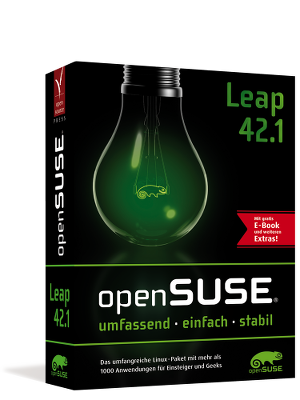
\includegraphics[width=0.34\textwidth]{openSUSE_sell}
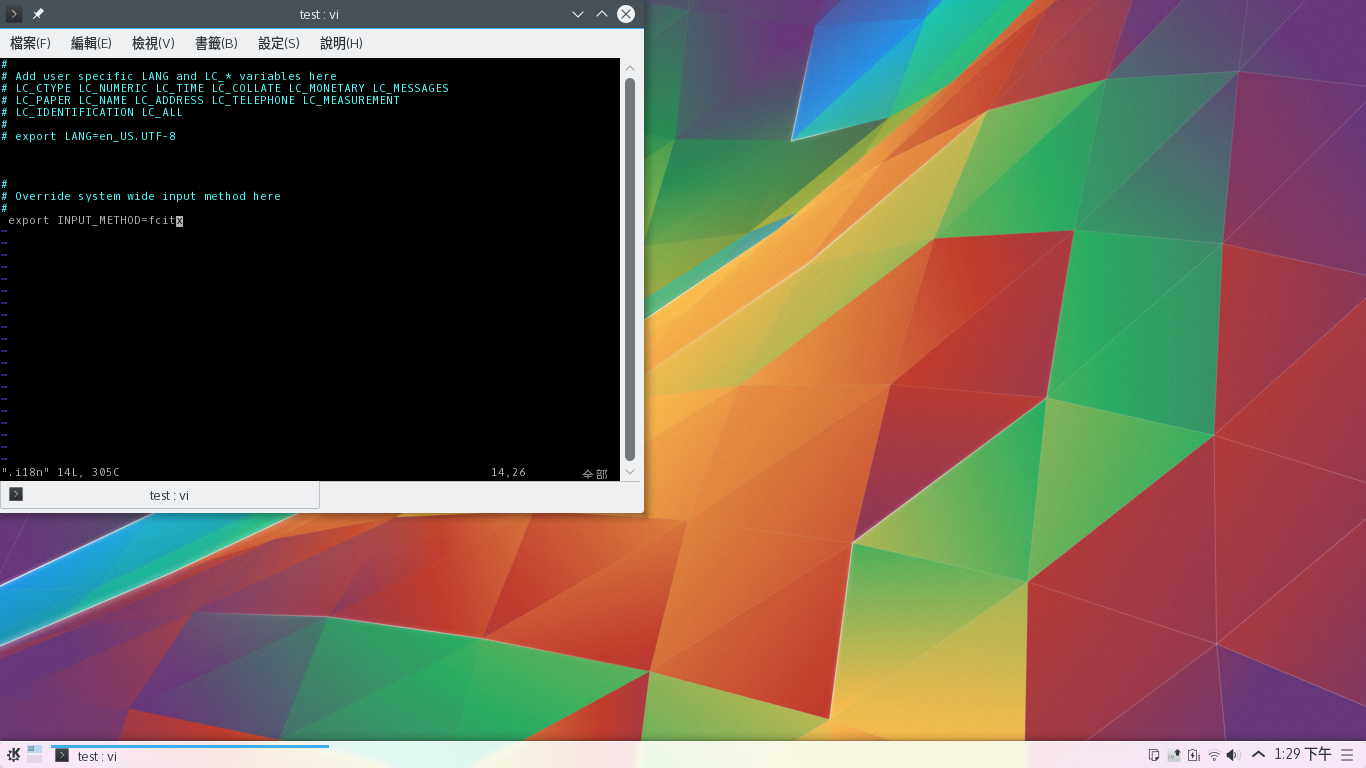
\includegraphics[width=0.66\textwidth]{opensuse_kde}

\begin{itemize}
  \item \textbf{优点:}非常健全并且直观的配置工具;非常齐全的软件源,十分出色的网站资源和文档。
  \item \textbf{不足:}和微软2006年关于专利和智慧财产权的协议,使得微软得以控制Linux,重量级的桌面设置和图形工具使得启动慢了一丢丢。
  \item \textbf{软件包管理:} Yast 图形和命令行管理工具,采用RPM封装包。
  \item \textbf{可选版本:} 32及64位版本(包括可安装的live CD 版本);针对i586,IA64,PowerPC,s390,s390x及x86\_64各个架构的企业桌面和服务器版。
\end{itemize}
%This statement requires citation \cite{book_key}; this one is more specific \cite[122]{article_key}.

%-----------------------------------------------------------------------
\section{生产力工具}\index{Tools in Linux}\index{Linux生产力工具}

本文介绍的工具绝大部分作者自己都常常使用因而比较熟练,有少部分作者认为非常好但是由于习惯或者工作
原因不常用,但是作者还是想介绍给大家,以便大家有多一个选择。
%-------------------------------------------------------
\subsection{Vim文本编辑器}\index{Vim}\index{Linux Vim}

\begin{center}

\includegraphics[width=0.7\textwidth]{vim-logo}
\end{center}

是的,Vim作为第一个出场,可见作者对其的重视和喜爱,作为一款强大高效的编辑器,堪称完美;
一旦你熟悉使用了它,我敢打赌,你会再也离不开它。实际上Vi是每个Linux版本的必备软件,Vim是Vi的加强
版,有些Linux版本默认安装,有些需要你自己安装。

你只需要你需要的,丢掉那些你不需要的,是的,就是这么极简。当然它还有极丰富强大的插件,
这里作者给出一些推荐。同时推荐用Vundle作为插件管理工具。

\begin{enumerate}
  \item ag.vim,使用它可以优雅的完成代码搜索和定位,速度飞快。\index{ag.vim}\index{Vim ag.vim插件}
  \item vimshell + vimproc,优雅的在Vim中完成各种终端命令CMD操作。\index{vimproc}\index{Vim vimproc插件}
  \item YouCompleteMe,使用YCM可以优雅的自动补全。\index{YouCompleteMe}\index{Vim YouCompleteMe插件}
  \item Ultisnip,优雅的增强YCM补全。而且可以自定义代码生成,简直神器。\index{Ultisnip}\index{Vim ultisnip插件}
  \item Multiple-Cursors,使用它可以优雅的完成多光标同时输入,实在是强。\index{Multiple-Cursors}\index{Vim Multiple-Cursors插件}
  \item tmux,终端分屏插件,可以让你同时在一个终端中打开几个窗口。\index{tmux}\index{Vim tmux插件}
\end{enumerate}

Vim是一个跨平台工具,它是我的常用文本编辑器,它的全键盘快捷操作能大大提升你的工作效率,
诚然它的入门不是那么直白易切入,不过花上点时间练习熟络它你会得到超值回报。
\begin{figure}[!th]
\noindent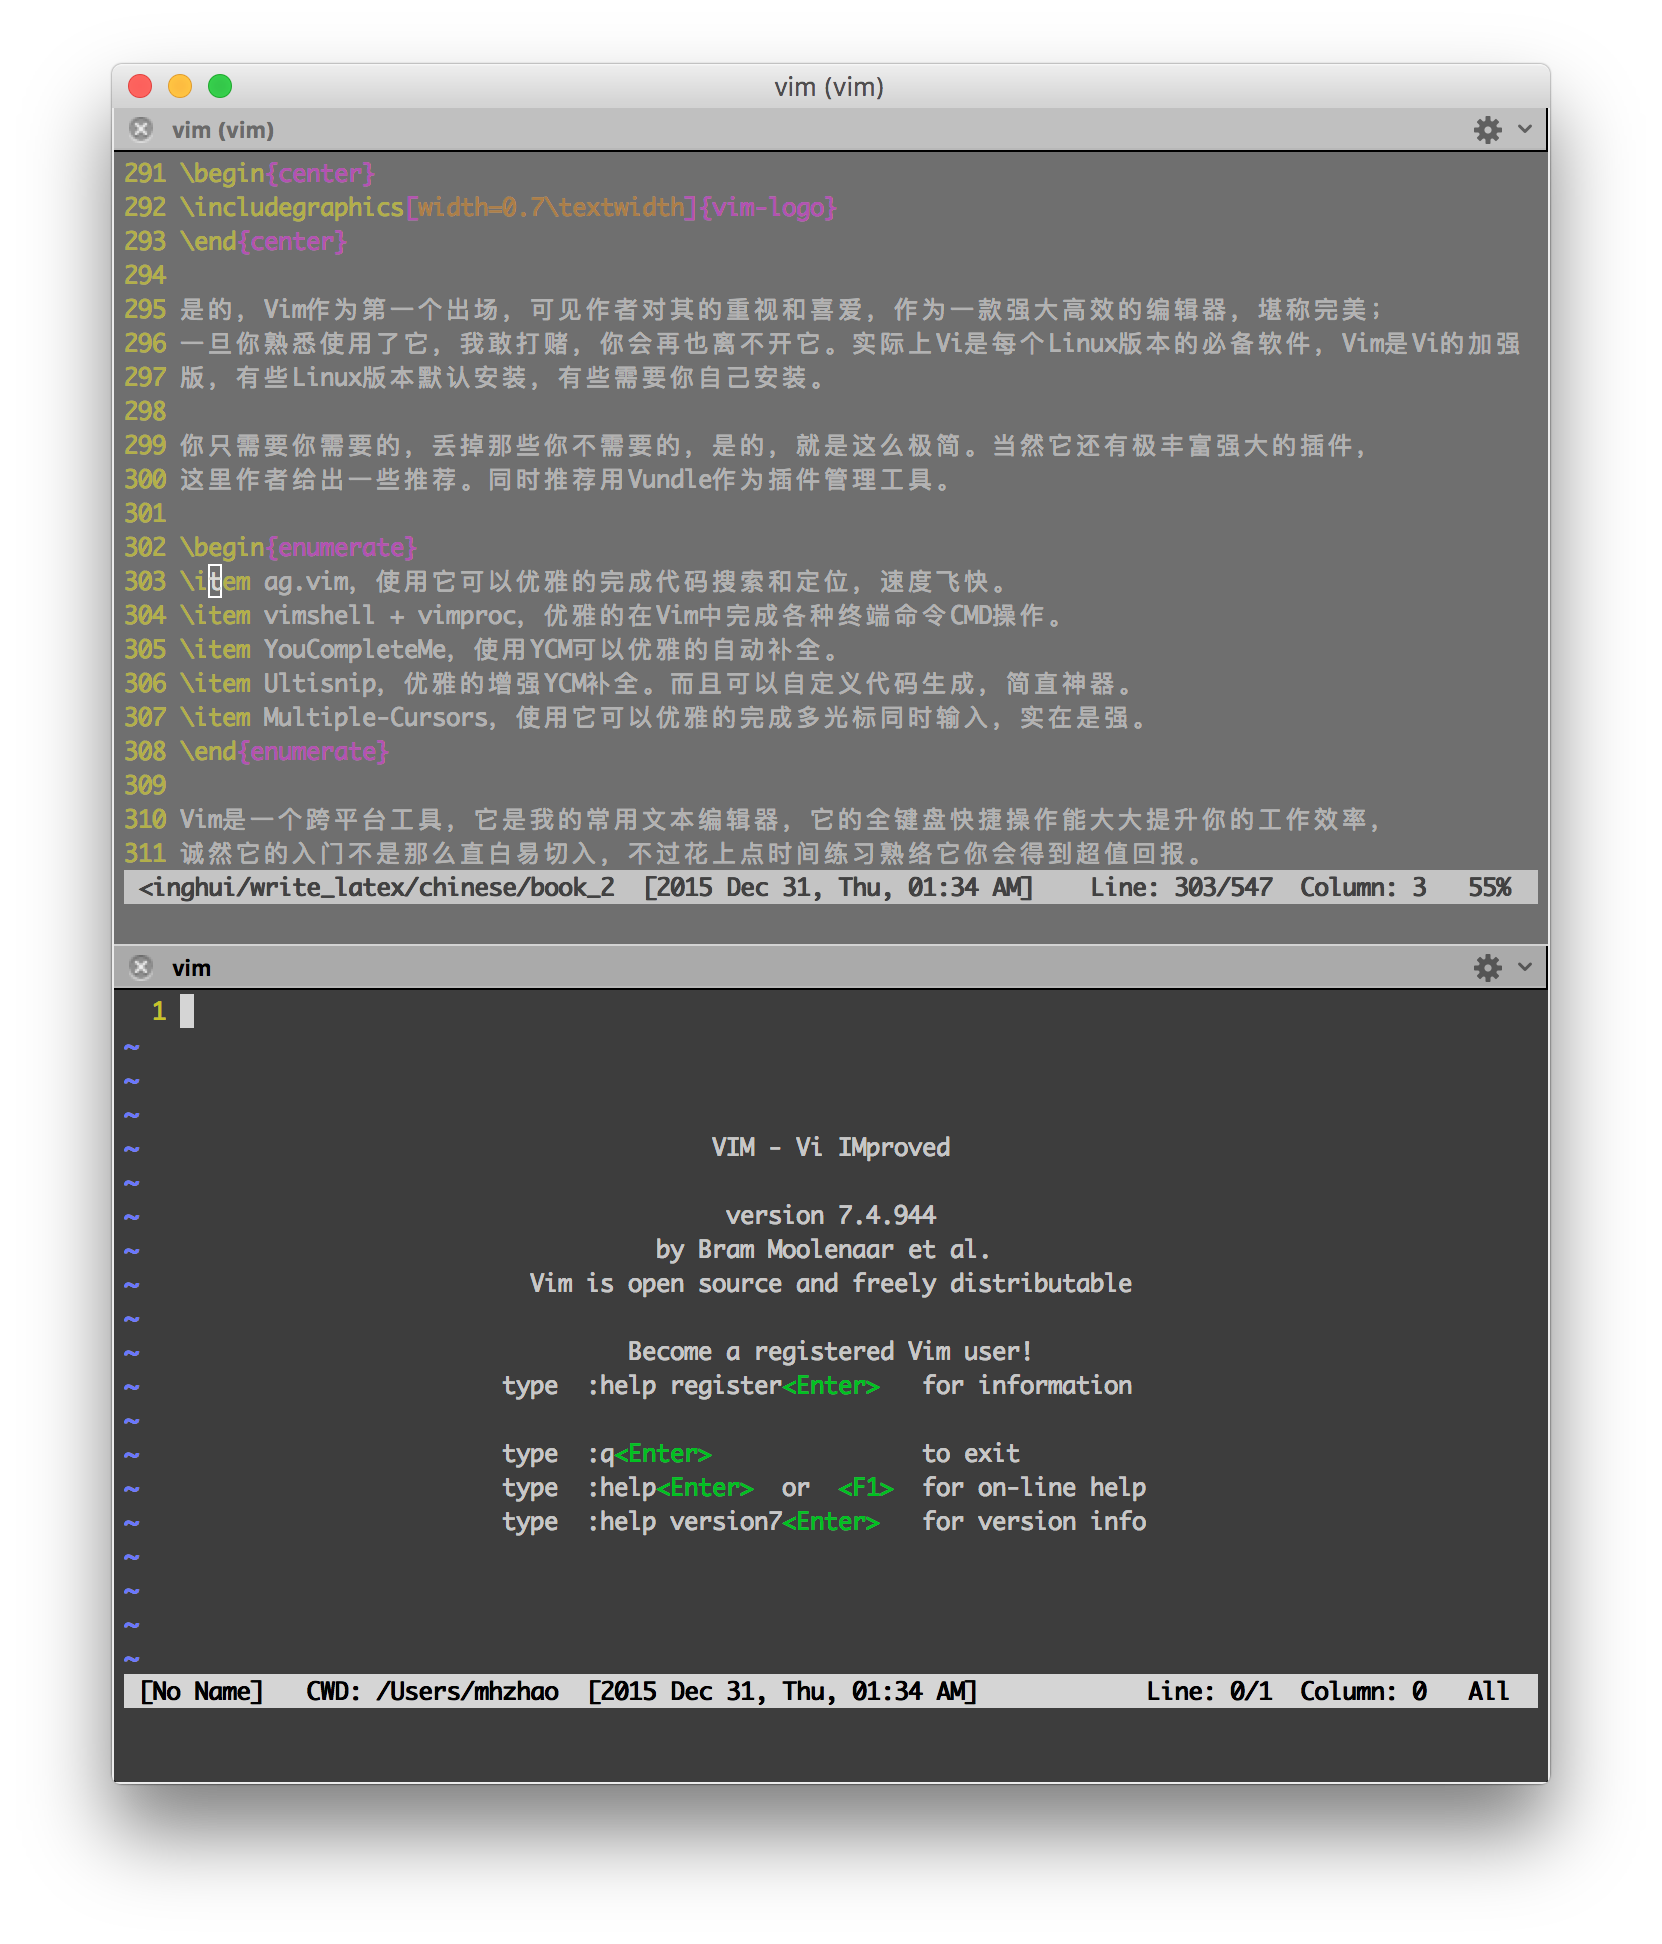
\includegraphics[width=1.0\textwidth]{vim-tool}
\caption{Vim打开界面(下)和工作编辑文档界面(上)}
\end{figure}
\begin{tips}
  一旦你习惯了Vim,很可能你会像我一样,干任何事都想用Vim来工作,比如编程,即使有非常好用的IDE环境
  ,我还是习惯性的默认使用Vim工作,当然有很多插件可以帮助你尽可能的实现各种IDE的功能,这时你就得
  花时间折腾了,而且很可能花费你不少的时间,有时候一时解决不了,让人特别沮丧,这都是正常的,我已
  经沮丧过很多次了。这里作者举个栗子,oh no,是例子\faOptinMonster。
\end{tips}
\begin{example}[vim-latexsuite插件安装]\index{vim-latexsuite}\index{Vim vim-latexsuite插件}
  我用的openSUSE 13.2版本,当时想用vim-latexsuite这个插件,在它主页上查了好久怎么安装使用,浪费了
  很多时间,后来发现在软件源里就有vim插件管理工具vim-addon-manager,查了manpage发现一下就能
  搞定,在安装了vim-latexsuite和vim-addon-manager后只需要在终端运行vim-addons install 
  vim-latexsuite就搞定了。
\end{example}

%-------------------------------------------------------
\subsection{Emacs文本编辑器}\index{Emacs}\index{Linux emacs}

\begin{center}

\includegraphics[width=0.5\textwidth]{Emacs-logo}
\end{center}

说了Vim,就不得不提Emacs,俩个类似的工具一直在争夺谁是文本编辑器届的No. 1,两方拥鳖也是各不相让,
我用惯了Vim,当然支持Vim,也许一开始学习Emacs,我现在就成了Emacs的粉丝了。是的,两者只要你最先
接触学习一个,就足以强大到吸引你不再甩另一个,也就是个先入为主的概念,学习任何一个都会让你一辈子
离不开。

\begin{itemize}
\item 和一样VIM一样,可以完整的全键盘操作,另外它的命令缓冲功能可以令你快速调用命令。
\item 更加灵活的可定制化以及超级丰富插件使得Emacs可以全能的胜任很多IDE环境。 
\item 学习曲线是渐进式的,对初学者相对友好。
\end{itemize}

\begin{figure}[!h]

  \noindent
  \begin{subfigure}{0.5\textwidth}
    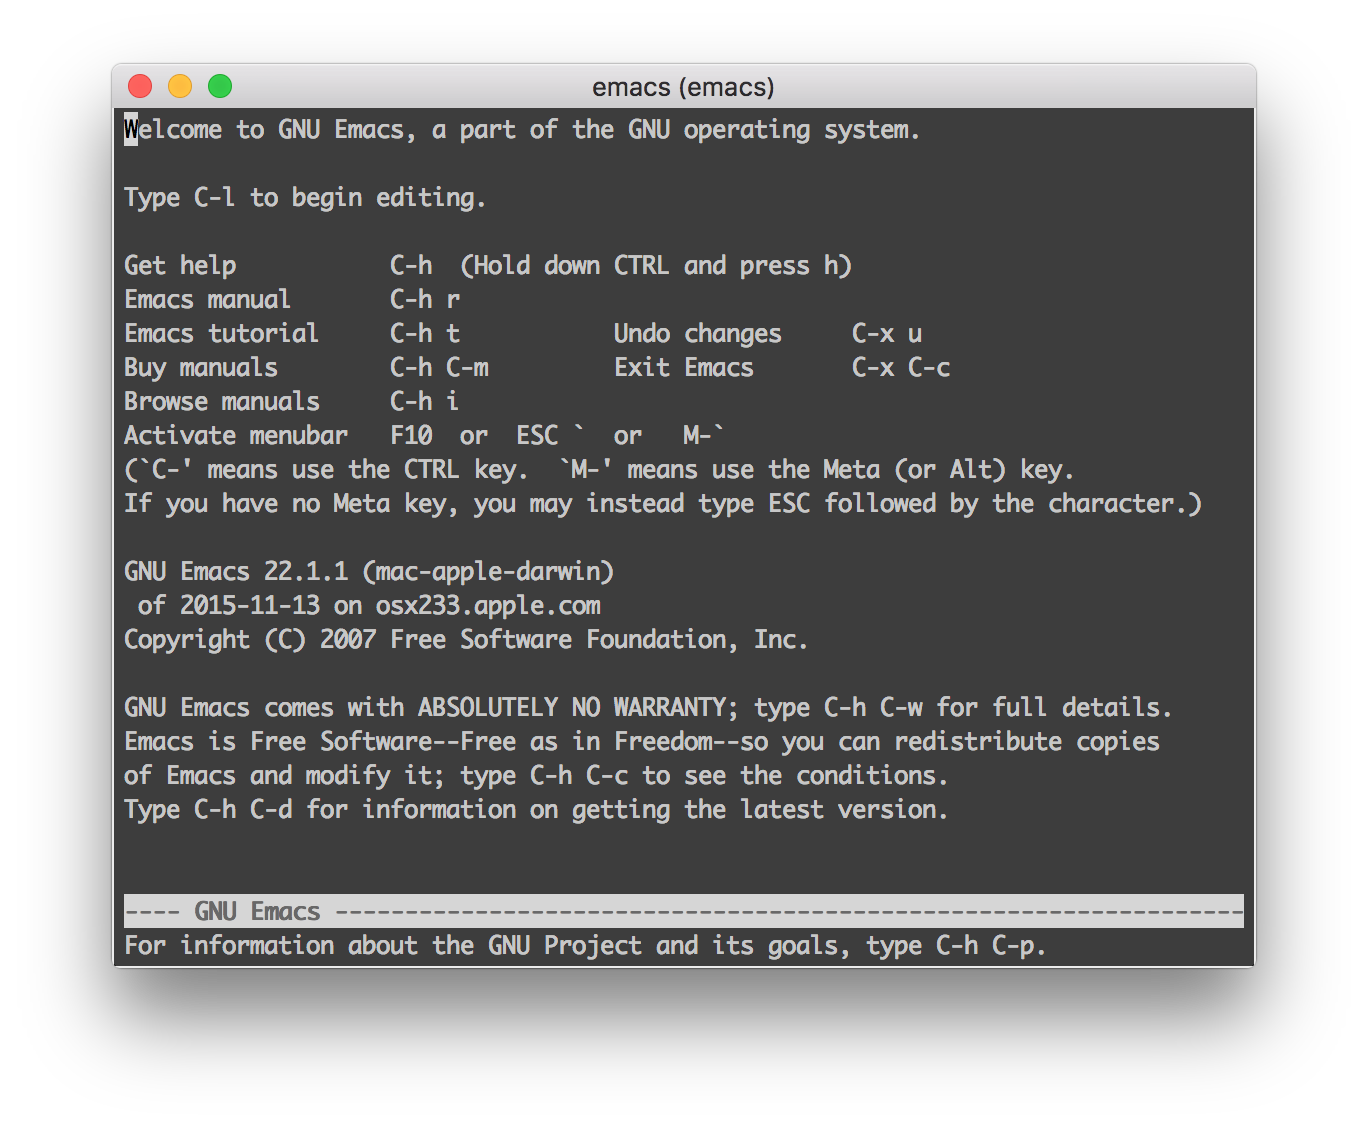
\includegraphics[width=1.10\textwidth]{emacs-nowindow}
    %\caption{emacs without window}
  \end{subfigure}
  \begin{subfigure}{0.5\textwidth}
    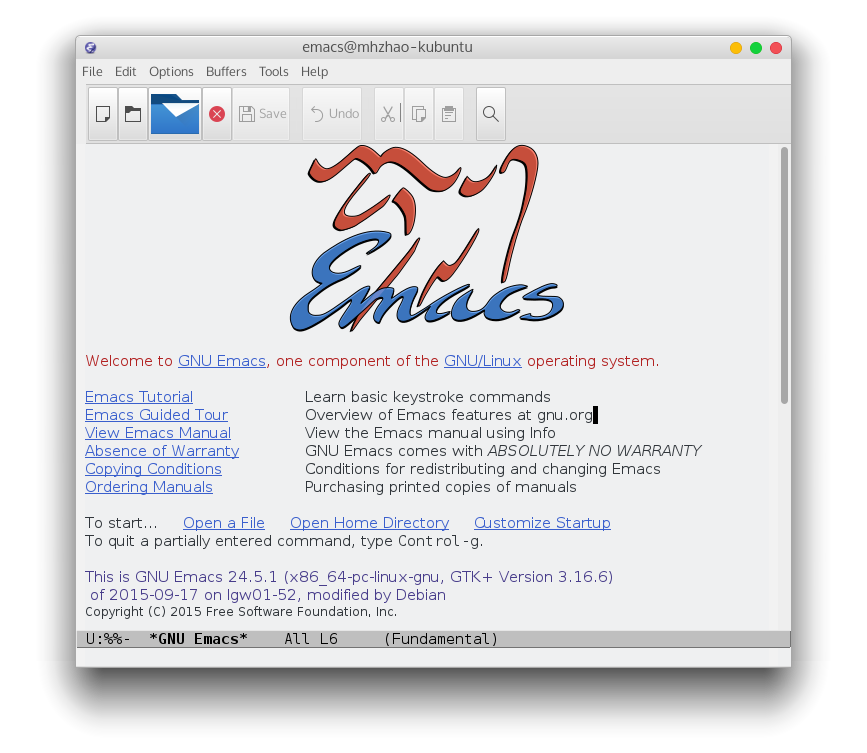
\includegraphics[width=0.97\textwidth]{emacs-windows}
    %\caption{emacs 图形界面}
  \end{subfigure}

  \caption{emacs 图形界面(右)和非图形界面(左)}
\end{figure}

%-------------------------------------------------------
\subsection{oh my zsh}\index{oh my zsh}\index{Linux oh-my-zsh}

\begin{center}

\includegraphics[width=0.5\textwidth]{ohmyzsh}
\end{center}

大部分Linux发行版本自带默认的shell为bash,也有少些默认为不同的shell,而且中zsh就是优秀的一款shell
,oh my zsh提供了管理zsh配置的框架,使得zsh跟用户互动更友好,超级丰富的插件,非常酷炫的主题,都是
你选择它的理由。
\begin{tips}
  shell是用户和Linux操作系统之间的接口。它是命令语言、命令解释程序及程序设计语言的
  统称 。 Linux中有多种shell,比如Bounrne shell, C shell, Korn shell, Bourne again shell, 
  Tenex C shell, Z shell等。大本分Linux版本缺省使用的是Bash。
\end{tips}
\begin{notation}\index{Prezto}\index{Linux Prezto}
  Zsh还有另外一个管理框架叫Prezto,它是oh my zsh的一个分支,改善了oh my zsh有迟滞感的速度慢的问题
  ,如果你不是特别需要回到oh my zsh的某个插件用法习惯,建议你使用Prezto,体验飞速的感觉真的很爽。
\end{notation}
%-------------------------------------------------------
\subsection{\LaTeX}\index{Linux \LaTeX}\index{\LaTeX}
\TeX 是一款文档排版软件,主要生成PDF格式的文档。\LaTeX 是为了减少用户难度而预设的\TeX 的宏的合集
,它有各种格式的预排版,因此用户不需要理会格式而只需要专注于内容就行了,省去了排版的时间和麻烦。
例如,本册就是用\LaTeX 生成的。

Linux下的\TeX 版本为\TeX Live,它包括了\TeX 相关的主要程序、宏包和字体。
\begin{center}
  
\includegraphics[width=0.5\textwidth]{Logo_TeX_Live}
\end{center}
在Linux系统中可以一键安装texlive-full,你就有了所有的应用程序、宏包和字体支持。有了宏包你就可以编
辑你的文档了,有很多很好的\LaTeX 编辑器可以帮助你大大提高效率,比如环境插入、命令补全、公式及特殊
符号应用、错误自动更正和定位等。
\begin{figure}[!h]
  \begin{subfigure}{0.19\textwidth}
    
\includegraphics[width=1.0\textwidth]{Kile}
  \end{subfigure}
  \begin{subfigure}{0.19\textwidth}
    
\includegraphics[width=1.0\textwidth]{Texstudio_Logo}
  \end{subfigure}
  \begin{subfigure}{0.18\textwidth}
    
\includegraphics[width=1.0\textwidth]{Texmaker_Logo}
  \end{subfigure}
  \begin{subfigure}{0.20\textwidth}
    
\includegraphics[width=1.0\textwidth]{TeXworks_icon}
  \end{subfigure}
  \begin{subfigure}{0.20\textwidth}
    
\includegraphics[width=1.0\textwidth]{lyx_logo}
  \end{subfigure}
  \caption{从左到右依次为Kile,TeXstudio,Texmaker,TeXworks,LyX}
\end{figure}
前文介绍的vim-latexsuite就是我的编辑器,是的,我离不开vim。上图的
一些集成环境编辑器也非常好,很强大,推荐kile,因为它可以设置成vim编辑器模式。

有了编辑器,你就可以快速高效的写作你文档了,不过你要写作书籍或者文章时就不得不和参考文献打交道,
不怕,Linux下有非常好大文献管理工具,例如Zotero,(k)BibTex,Jabref,Mendeley等。Zotero是Firefox的
插件,其它的都是独立的软件。像Jabref和Mendeley都是跨平台的,Mendeley的功能更强大些,它可以兼容
Microsoft Word, LibreOffice和BibTex。这里作者推荐Jabref和Mendeley。
\begin{figure}[!h]
  \begin{subfigure}{0.24\textwidth}
    
\includegraphics[width=1.0\textwidth]{Zotero_logo}
  \end{subfigure}
  \begin{subfigure}{0.24\textwidth}
    
\includegraphics[width=1.0\textwidth]{Kbibtex-icon}
  \end{subfigure}
  \begin{subfigure}{0.24\textwidth}
    
\includegraphics[width=1.0\textwidth]{JabRef_Icon}
  \end{subfigure}
  \begin{subfigure}{0.24\textwidth}
    
\includegraphics[width=1.0\textwidth]{Mendeley_Logo}
  \end{subfigure}
  \caption{从左到右依次为Zotero,KBibTex,JabRef,Mendeley}
\end{figure}

%-------------------------------------------------------
\subsection{Video、Audio、Picture多媒体编辑}\index{Linux多媒体编辑}

%-------------------------------------------
\subsubsection{Desktop录制工具}\index{Linux桌面录制工具}

\includegraphics[scale=0.3]{Open_Broadcaster_Software_Logo}
  Open Broadcaster是一款非常优秀的开源跨平台的实时视频流和录制软件,非常好用而且功能很强大,是很
  多游戏玩家录制的首选,用来录制桌面显得有些大材小用了。它同时是我在Windows以及Mac OS上喜爱用的
  工具。

  
\includegraphics[scale=0.15]{vokoscreen}
  Vokoscreen也是一款Linux下非常强大的桌面录制软件,有openSUSE、Ubuntu、Debian版本,它是专门为
  录制桌面以制作视频教程而开发的简单易用的桌面录屏软件。它是我在Linux下最喜爱用的录制桌面视频
  工具。

%-------------------------------------------
\subsubsection{Video播放及编辑工具}\index{Linux视频播放及编辑工具}
\begin{figure}[!h]
  \begin{subfigure}{0.24\textwidth}
    
\includegraphics[width=1.0\textwidth]{VLC_Icon}
  \end{subfigure}
  \begin{subfigure}{0.24\textwidth}
    
\includegraphics[width=1.0\textwidth]{Kaffeine}
  \end{subfigure}
  \begin{subfigure}{0.24\textwidth}
    
\includegraphics[width=1.0\textwidth]{Mpv_icon}
  \end{subfigure}
  \begin{subfigure}{0.24\textwidth}
    
\includegraphics[width=1.0\textwidth]{Miro_icon}
  \end{subfigure}
  \caption{从左到右依次为VLC,Kaffeine,MPV,Miro player}
\end{figure}
虽然Linux有很多视频播放器,很多都很好,不过,最流行(之一)的一款就是VLC了。一般自带的播放器都
足够好了,如果你需要再多一款的话选VLC就足够了,VLC是一款优秀的跨平台多媒体平台,作为功能之一的播
放器,几乎支持所有格式的视频解码,非常强大好用。

Linux下的开源视频编辑工具选择很多,比如Pitivi、Cinelerra、Kino、Avidemux、LiVES、OpenShot等,不过
这里推荐Kdenlive和Blender。
\begin{itemize}
  \item 
  
\includegraphics[width=0.2\textwidth]{Blender}
Blender作为一款非常强大等3D视频编辑器,名声上蹿很快,在电影工业中应用也越来越多。
  \item 
  
\includegraphics[width=0.05\textwidth]{Logo-kdenlive}
Kdenlive相较于其他视频编辑器支持的场景是最多最全的。
\end{itemize}

%-------------------------------------------
%-------------------------------------------
\subsubsection{Audio播放及编辑}\index{Linux音频播放及编辑}
对于音频播放器基本默认自带就足够了,比如banshee、Rhythmbox、Amarok等,当然前面提到的视频播放器也
包括了音频播放功能。对于音频编辑工具选择也很多,这里推荐一个Audacity就足够用了。
\begin{itemize}
  \item 
\includegraphics[width=0.1\textwidth]{Audacity_Logo}
    Audacity不仅能够录制多轨音频,而且支持各种音频格式的后期处理。一些音乐专辑就是用它制作的。
\end{itemize}
%-------------------------------------------
\subsubsection{Picture编辑}\index{Linux图片编辑}
这里还是推荐用系统自带的图片和照片管理工具,因为已经都好了,对于图片制作和编辑GIMP和Inkscape就能
满足绝大部分人的需求。


\includegraphics[width=0.05\textwidth]{Wilber-gimp}
GIMP和Photoshop一样强大,嗯,说这么多就够了。


\includegraphics[width=0.05\textwidth]{Inkscape_Logo}
Inkscape是一款矢量作图软件,用它发挥你的才华和创意吧。
\begin{recommendation}[photo managers or editors]
  \begin{itemize}
    \item
    \item digiKam:摄影师的好伴侣,脸部识别功能很赞。
    \item darktable:摄影师之友,更专业的艺术特征支持,开始上手有点难。
    \item Fotoxx:最好用的工具之一,可以添加自己的特效,艺术照转换。
    \item F-Spot:非常简单易上手。
    \item GTKRawGallery:支持Dropbox上传,支持后台运行。
    \item Pixeluvo:强大易用,界面漂亮。
  \end{itemize}
\end{recommendation}
%-------------------------------------------------------
\subsection{Office办公}\index{Linux办公软件}
说到办公软件,你想到了什么?反正在我脑海里就是处理处理文档。微软Office是最常见最不可缺少的办公软
件,大家印象里好像除了微软Office没有其它的选择。但是,Linux下的自由软件给大家带来了不同选择。

\includegraphics[width=0.2\textwidth]{LibreOffice_Logo}
Linux下有影响力的办公软件非LibreOffice莫属,而且它是跨平台的,虽然不像微软Office那样熟悉丰富,不
过作为办公软件它还是胜任的。

\includegraphics[width=0.2\textwidth]{WPS_office_logo}
中国的金山出品的WPS Office也是一套完整的办公套件,有免费的个人版 提供,不过我用了几次Linux版的,
启动有点慢,还经常卡着不动,就卸了。

%-----------------------------------------------------------------------
\section{其它常用工具}\index{Linux其它工具}

\subsection{Math数学工具}\index{Linux数学工具}
虽然专业的商业软件很多也有Linux版,比如Mathematics、MATLAB等,但是在Linux也有非常优秀的替代品,
虽然它们赶不上商业软件美观好用,但是对于基本需求上的使用上并不差。比如简单的数据画图,我用gnuplot
就能满足我的大部分需求,再比如做作业时数学符号计算或者数值计算上Maxima也基本满足我的需求。这里列
举了一些流行的Linux下的数学工具。
\subsubsection{Gnuplot画图软件}\index{Linux gnuplot画图}
这个真的很好用,而且它的脚本语言简单的一塌糊涂,而且它有完善的帮助文档,交互界面也非常友好,可以
快速达到你的作图要求。网上有很多很多它的入门教程,基本上半个小时你就能入门了,如果你愿意花两个小
时,你就能精通它了,它的自助文档系统非常强大友好简单易懂。

Gnuplot作为一个命令行工具,也有非交互的脚本支持,都能让你如愿可视化你的数学函数或者数据,而且它也
成为许多第三方数学工具的画图引擎,比如Octave,Sage等。
\subsubsection{SageMath数学软件系统}\index{Linux SageMath数学软件}

\vspace{0.5cm}
\begin{center}
  \includegraphics[width=0.5\textwidth]{Sage_logo_new}
\end{center}

SageMath简直是一个数学系统,它力图涵盖数学相关的所有方面,比如,几何、微积分、数值计算、图形、数
论等等。它的目标是做一个替代Magma,Maple,Mathematica和Matlab的免费开源工具。
\subsubsection{Maxima数学符号计算}\index{Linux Maxima数学软件}
\begin{center}
  \includegraphics[width=0.15\textwidth]{Maxima-new}
\end{center}

\vspace{-0.1cm}
Maxima是一款类似于Mathematica的数学软件,主要强项在于符号计算,当然也可以用于数值计算,它的画图引
擎用的是Gnuplot,它既可以命令行端交互,也有图形前端,如果你不想花钱买Mathematica,用Maxima也是不
错的选择,虽然没有Mathematica那么美观好用,但是基础需求还是能满足的。
\subsubsection{R统计计算}\index{Linux R数学统计软件}
由于领域的原因我并没有用过这个软件,它是专门为统计计算和数据分析及图形化展示数据的软件。我下学期选
的Machine Learning课要用它,待我学了再回头说它。
\subsubsection{Octave和Scilab数值计算}\index{Linux Octave和Scilab数学软件}
这两个功能重叠性非常高,都擅长于数值计算处理,二者都是为寻求MATLAB替代者而生。Octave兼容MATLAB文
件更好一些,它的语法和MATLAB几乎一摸一样。但是二者中作者跟推荐Scilab,不只是因为Octave没有图形界
面而Scilab有,而是因为Scilab功能更多更强大。
\subsubsection{GeoGebra图形软件}\index{Linux GeoGebra数学图形软件}
嗯,这是一款非常有用的数学软件,它在数学各种图形的制作上非常强大,而且它的使用对象从小学生到大学
研究生老师无所不包。它不只是数学工具,还有其它丰富的功能,比如地理上也可以应用,它甚至在
Kickstarter进行了筹资以开发iPad和Android版本。目前它的扩长非常迅速。
\subsubsection{\LaTeX 和Lurch数学文档处理}\index{Linux \LaTeX 和Lurch数学文档处理软件}
很多人为编辑数学公式时的低效笨拙而苦恼过,这两个工具就能很好的解决这个问题,特别是Lurch,专门为了
数学公式而开发的,可以支持\TeX 模式,给个赞。
\begin{tips}
  ROOT是我专业上常用的数据处理软件,实际上它还是一个编程框架,还有自己的编译器,可以运行C++脚本
  语言,也可以正常的面向对象的C++编程,它有非常强大丰富的数学库,数据处理和画图都不在话下。
\end{tips}
\subsection{Program编程工具}\index{Linux编程工具}
由于我编程项目都不大,所以不怎么用集成开发环境,对于一些IDE工具并没有体验,在Linux下我都用gcc编译
器,不过我专业的关系,要用ROOT做数据处理,所以介绍下ROOT吧,不过下面会列出一些经常见到的IDE。

\vspace{-2.2cm}
\begin{figure}[!h]
  \centering
  \begin{subfigure}{0.4\textwidth}
    \includegraphics[width=0.8\textwidth]{rootlogo-old.pdf}
  \end{subfigure}
  \begin{subfigure}{0.45\textwidth}
    \includegraphics[width=0.90\textwidth]{logo_root}
  \end{subfigure}
  \vspace{-1.8cm}
  \caption{ROOT旧Logo(左)和新Logo(右)}
  %\label{fig:root}
\end{figure}

\begin{recommendation}[IDE for programming]
  \begin{itemize}
    \item
    \item Eclipse:支持语言Java, C, C++, PHP, Python, Perl, Ruby and more;各种功能插件扩展。
    \item Bluefish:支持语言ASP .NET, C/C++, CSS, HTML5, JavaScript and jQuery, Java, Pearl, PHP, 
      Ruby, SQL, WordPress, and XML。
    \item kDevelop:支持语言C/C++, PHP和Ruby;支持KDE/QT开发。
    \item NetBeans:支持语言Java, Python, C/C++, Ruby, PHP, JavaScript等。
    \item Code::Blocks:支持语言C, C++ and Fortran。
    \item CodeLite:支持语言C and C++。
  \end{itemize}
\end{recommendation}
%----------------------------------------------------------------------------------------
%	CHAPTER 2
%----------------------------------------------------------------------------------------

\chapterimage{os-x-el-capitan} % Chapter heading image
\chapter{Mac \texorpdfstring{\faApple}{world}}\index{Mac}
\section{系统设置}\index{Mac 系统设置}
第一感觉,苹果系统慢。我的价值2000多刀的Macbook Pro 2014版15寸的最高配,但是用起来还没有400多刀的
Dell Inspiron 7437 i5处理器(我自己换了SSD硬盘)跑的openSUSE 13.2 KDE快。第二感觉,苹果系统用起来
麻烦。苹果系统自己设置了很多很复杂(起码一个手吃力)的快捷键,简直是反人类设计,而且如果想自己设
置一些快捷键不但复杂,而且大量组合键不能用,必须复杂的两个以上功能键组合,真是反人类反到没天理。
好吧,以上这些都是我用惯了Linux系统,而且从来不用鼠标,都是全键盘操作,可以自己快速定制简单的快捷
键后造成的印象。虽然苹果系统用起来不够畅快,但是它美呀,不但硬件美,而且系统UI界面也很美,我一直
想把它卖了,但是为了它的美和独一无二(作为一个科技迷不能不会用苹果操作系统吧)还是忍着留下来了。
当然,苹果系统也有它让人割舍不下的功能和体验,比如,集成于系统的搜索和词典功能,好用的触摸板功能
等等,总之,没有什么东西是完美的,好不好用主要取决于它怎么满足于你的需求,但是我们可以做一些设置
,使它更完美。

为了更好用,有必要对苹果系统进行一些设置,比如我根本就不用鼠标,所以要设置触摸板上模仿鼠标的行为
,还要设置一些常用的快捷键,系统设置上的限制,使得我们不得不借助于一些第三方工具。下面主要是介绍
一些第三方应用,至于系统层面的设置,苹果给出的都是选择题,对你来说没啥难度。

由于非常多优秀的优秀软件都是收费的,而本文主要介绍的是免费开源应用,前文介绍的Linux版应用几乎都有
对应的Mac版本,而且支持都非常好,再加上到目前为止作者还没用苹果系统多久,所以关于苹果系统相关软件
的介绍不多,以后随着使用的增加会慢慢增加这部分的介绍。
\subsection{BetterTouchTool}\index{Mac BetterTouchTool}\index{BetterTouchTool}
  \includegraphics[width=0.05\textwidth]{BBTlogo}
  这是一个fantastic工具,可以让你随心所欲定制你的触摸板功能,比如在系统设置层面并没有模仿鼠标中键
  选项,这里就可以添加,再比如你可以搭配一个功能键加触摸板去设置一些你想要的弄能或者快捷操作,加
  上键盘快捷键的定制,当然还有更多弄能设置,总之,它简直是摆脱鼠标的利器。它的设置界面如图所示。
  
  \vspace{-0.5cm}
  \begin{figure}[h]
    \centering
    \begin{subfigure}{1.0\textwidth}
      \includegraphics[width=1.0\textwidth]{bettertouchtrackpad}
    \end{subfigure}
    %\begin{subfigure}{0.5\textwidth}
    %  \includegraphics[width=1.0\textwidth]{bettertouchkeyboard}
    %\end{subfigure}
    \caption{BetterTouchTool的设置界面,图中是我添加的触摸板模仿鼠标中键功能}
    %\label{fig:<+label+>}
  \end{figure}
  \begin{recommendation}{Mac快捷键推荐}\index{Mac快捷键推荐}
    \begin{itemize}
        \item
      \item Alt/Option + A:应用程序窗口桌面左半边最大化。
      \item Alt/Option + L:应用程序窗口桌面右半边最大化。
      \item Alt/Option + F:打开文件管理器Finder。
    \end{itemize}
  \end{recommendation}
\begin{notation}
  BetterTouchTool并不是一款开源软件,但是它是免费的。就在刚刚收到开发者 的信息说,他很可能决定
  把它变成收费软件了,oh no\dots
\end{notation}

\subsection{Homebrew}\index{Mac Homebrew}\index{Homebrew}
苹果和Linux作为Unix系统分支,我们可以完全在苹果系统上实现Linux的各种功能和软件配置。这大大方便了
我的工作,是的,我的一切工作又回到了终端中。这一切要归功于Homebrew软件,Homebrew就像Linux下的软件
源管理软件一样,它提供了丰富的软件,可以非常简单的搜索、安装和卸载。建议一定安装这个,方便你管理
各种开源软件安装。
\begin{tips}
  MacPorts是另一个Mac系统下的软件源管理软件,如果你熟悉BSD系统,那么用MacPorts,跟Homebrew相比,
  MacPorts的软件更丰富,它的库里现在有2万5千多款软件可选,你几乎能找到任何你想要的开源软件。
\end{tips}

\section{生产力工具}
到目前为止,我发现的Mac下最好的软件都是商业软件,所以我的一切配置都是按照Linux来配置的相应的软件
感觉没啥可介绍的了。
\subsection{TextWrangler}\index{Mac TextWrangler}\index{TextWrangler}
由于TextMate和Sublime变为收费软件,TextWrangler作为免费好用的文本编辑器,可以试一试。
\subsection{NeoOffice}
\begin{center}
  \includegraphics[width=0.1\textwidth]{NeoOffice_icon}
\end{center}
它是openoffice的Mac版,当然其它openoffice的分支也有Mac版,如libreoffice和apache office,不过
NeoOffice是专门为Mac开发的。
\subsection{其它工具推荐}\index{Mac其它工具推荐}
正如我上面所说,我基本沿用了Linux下的工作工具,前面Linux下介绍的所有的软件和工具都有对应的Mac版本
,我用Homebrew作为管理工具,通过它安装了我所需要的软件。然后我做的配置几乎和我的Linux工作环境一样
,下面是我的工作是界面。这里我用的终端是iTerm是zsh,并且用了oh my zsh作为插件管理, 用了 tmux插件
。

\begin{recommendation}[我的软件列表]\index{Mac我的免费软件列表}
  \begin{itemize}
    \item 
    \item VLC:视频播放。
    \item iTerm:终端。
    \item Mac\TeX :latex编译系统。
    \item VIM:文本编辑器工具。
    \item Maxima:数学软件。
    \item Gnuplot:画图软件。
    \item Blender:视频编辑软件。
    \item Audacity:音频编辑软件。
    \item Google Chrome:浏览器。
    \item \TeX studio:latex编辑器。
    \item LyX:latex编辑器。
    \item OBS:桌面录制工具,全名为Open Broadcaster Software。
    \item TigerVNC Viewer:远程登录桌面查看器。
    \item GIMP:图片编辑器。
    \item Inkscape:图片编辑器。
    \item Scibus:电子杂志书籍制作软件。
  \end{itemize}
\end{recommendation}

\begin{figure}[h]
  %\centering
  \hspace{-0.6cm}\includegraphics[width=1.1\textwidth]{mac-work1}
  \caption{我的Mac工作界面1}
  %\label{fig:<+label+>}
\end{figure}
\begin{figure}[h]
  %\centering
  \hspace{-0.6cm}\includegraphics[width=1.1\textwidth]{mac-work2}
  \caption{我的Mac工作界面2}
  %\label{fig:<+label+>}
\end{figure}
%------------------------------------------------

%----------------------------------------------------------------------------------------
%	CHAPTER 3
%----------------------------------------------------------------------------------------

%\chapterimage{chapter_head_1.pdf} % Chapter heading image
\chapterimage{Windows-10-Official-Wallpaper} % Chapter heading image

\chapter{Windows \texorpdfstring{\faWindows}{world}}\index{Windows系统}
到这里我发现没啥可写了,以前没有Mac,所以电脑装了openSUSE 13.2和Windows 10双系统,偶尔还进入
windows系统登一下QQ或者偶尔玩下游戏,现在有了Mac,再也没借口和动机登windows系统了,基本弃用了。
所以这一部分就补充一下前面遗忘的一些软件吧。
\section{系统设置}\index{windows 系统设置}
也许windows 10本身就是更先进的生产力工具,因为windows 10确实优化了很多,用起来比以前畅快了很多,
它的搜索功能和Mac一样强大,尤其我用起来语音助手小娜感觉很好用。
\section{生产力工具}
\subsection{Evernote}\index{Evernote}
Evernote是一款笔记及管理和归档的软件,它有Mac和Windows版,最基础的版本是免费的,高级功能是收费的
,大家都反映说很有用且好用。
\subsection{OneDrive}\index{windows OneDrive}\index{OneDrive}
windows自己的云备份软件,容量有限,但是系统自带,好用。
\section{更多软件推荐}\index{Windows更多软件推荐}\index{Linux更多软件推荐}\index{Mac更多软件推荐}
\begin{itemize}
  \item Dia:流程图画图软件。
  \item $\mu$torrent: P2P下载软件。
  \item FileZilla: FTP软件。
  \item FreeMind和XMind:思维构图软件。
  \item BleachBit: Linux下的系统清理软件。
  \item MPlayer:视频播放器。 
  \item Skype:聊天视频及电话软件。
  \item Deluge: BitTorrent软件。
  \item CrashPlan: 备份软件。
  \item PeaZip: zip解压软件UI版。
  \item Wine: Linux下运行windows程序的环境模拟器。
  \item VirtualBox: 虚拟机,可以运行其它系统。
  \item Shotwell: 照片管理软件。
  \item Clementine: 音乐播放器。
  \item BitDefender: Linux下的反病毒软件。
  \item Thunderbird: 邮件管理软件。
  \item TestDisk和Safecopy: 文件数据恢复软件。
  \item Remote Desktop Manager: 远程登录桌面管理软件。
  \item Terminals: 远程登录桌面管理软件。
  \item mRemoteNG: 远程登录桌面管理软件。
\end{itemize}
\section{开源软件查找网站}\index{Open Source开源软件查找网站}
在这里 \textcolor{blue}{\url{http://sourceforge.net}} 你可以找到所有开源软件所有系统的版本。
\section{后记}
由于马上开学了,所以到最后Mac和Windows就草草结束了。而且发现分系统的组织结构问题很多,因为开源软
件基本都是三个平台都支持的,但是由于时间的关系没精力和时间去调整了。不过,终于把想法付诸实践了,
虽然不是很好,但是整个winter break总算做了点事,而不是又睡了三周。写点东西主要是督促自己不要浪费
时间,就算很简单的事不去做也是什么也得不到,不以硅步无以至千里,把小事特简单的事别人不以为是的事
做好就是进步,凡事都是开头做点容易,想要坚持下去真的是很难。能坚持下去的事都要兴趣支持,自己的小
爱好发展下去也许能超越职业发展。

上面两节很明显不是这一章的内容,本来计划Mac和Windows这两章应该像Linux那一章一样翔实,然后后面还有
两章分别为Write After Finishing后记和Bibliography引用两章,但是没有了,所以到此结束。

本册只是泛泛的列举,没有具体深入的介绍。以后有时间打算写一些深入的技术细节,包括系统和软件的具体
设置配置和使用,希望能践行落实。
%------------------------------------------------

%----------------------------------------------------------------------------------------
%	BIBLIOGRAPHY
%----------------------------------------------------------------------------------------

%\chapterimage{chapter_head_2} % Chapter heading image
%\chapter*{Bibliography}
%\addcontentsline{toc}{chapter}{\textcolor{ocre}{Bibliography}}
%\section*{Books}
%\addcontentsline{toc}{section}{Books}
%\printbibliography[heading=bibempty,type=book]
%\section*{Articles}
%\addcontentsline{toc}{section}{Articles}
%\printbibliography[heading=bibempty,type=article]
%\item 

%----------------------------------------------------------------------------------------
%	INDEX
%----------------------------------------------------------------------------------------

\cleardoublepage
\phantomsection
\setlength{\columnsep}{0.75cm}
\addcontentsline{toc}{chapter}{\textcolor{ocre}{Index}}
\chapterimage{chapter_head_1} % Chapter heading image
\printindex

%----------------------------------------------------------------------------------------

\end{document}
